\newcommand{\alohaAccuracyTrend}{
    \begin{figure}[H]
        \vspace*{-0.5cm}
        \centering
        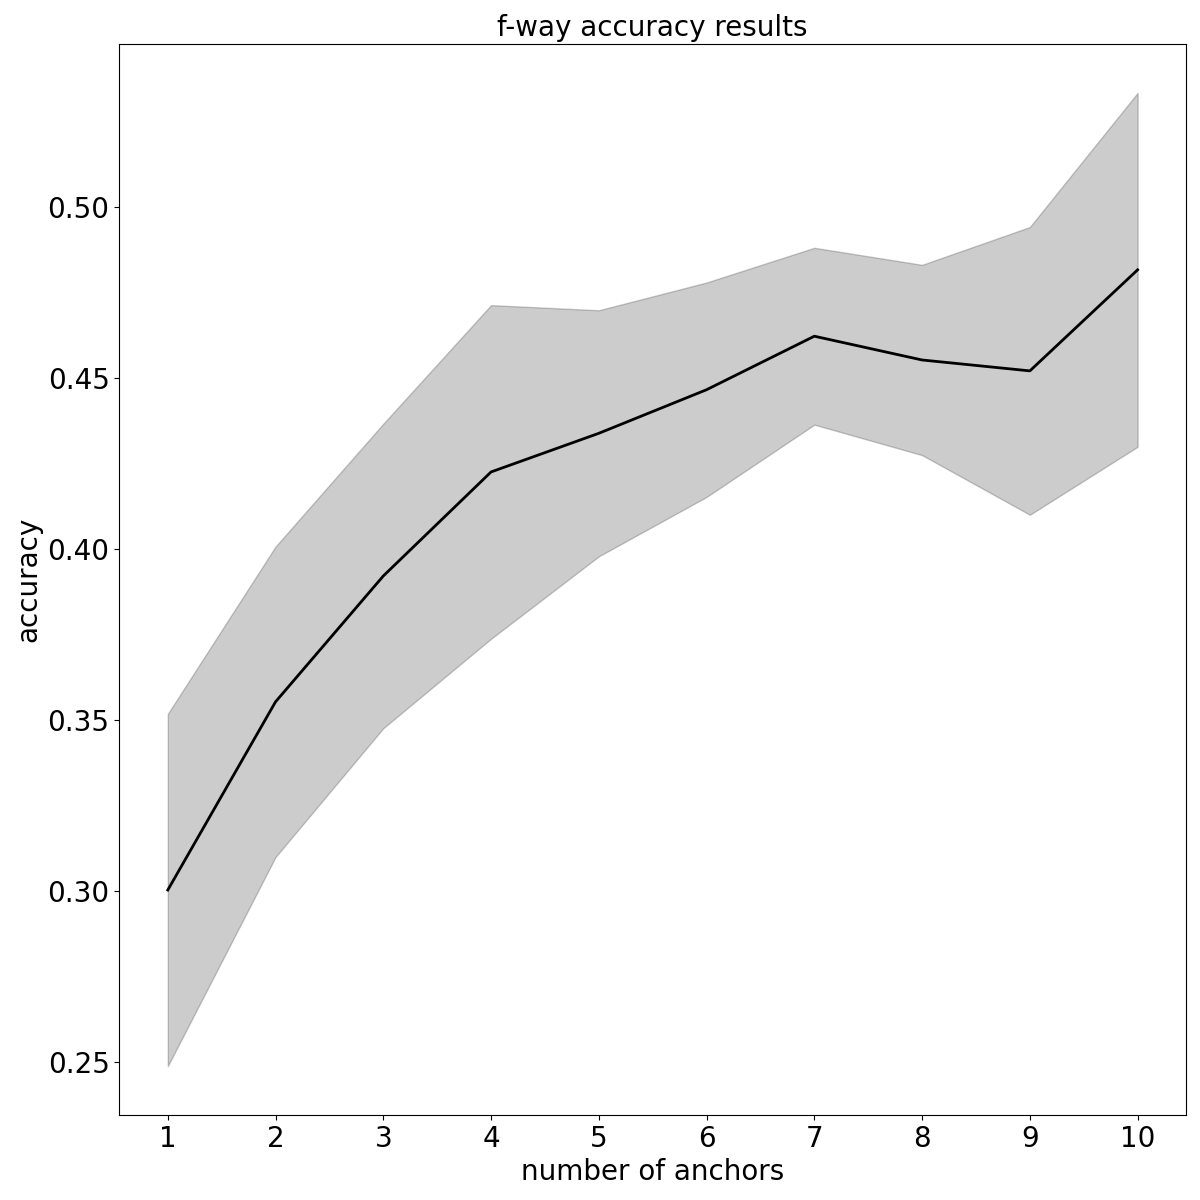
\includegraphics[width=0.65\textwidth]{./results/accuracy_trend_aloha.png}
        \vspace*{-0.2cm}
        \caption[ALOHA Family Prediction Accuracy Trend]{\textBF{Accuracy Trend} (varying the number of anchor samples used) resulting from the evaluation of the \textBF{ALOHA} implementation on the Malware Family Prediction task. The line represents the \textit{mean} Accuracy, while the shaded region represents the \textit{standard deviation}. Statistics were computed over 15 evaluation of the same model with different query and anchor samples.}
        \label{fig:alohaAccuracyTrend}
    \end{figure}
}

\newcommand{\alohaMBAccuracyTrend}{
    \begin{figure}[H]
        \vspace*{-0.5cm}
        \centering
        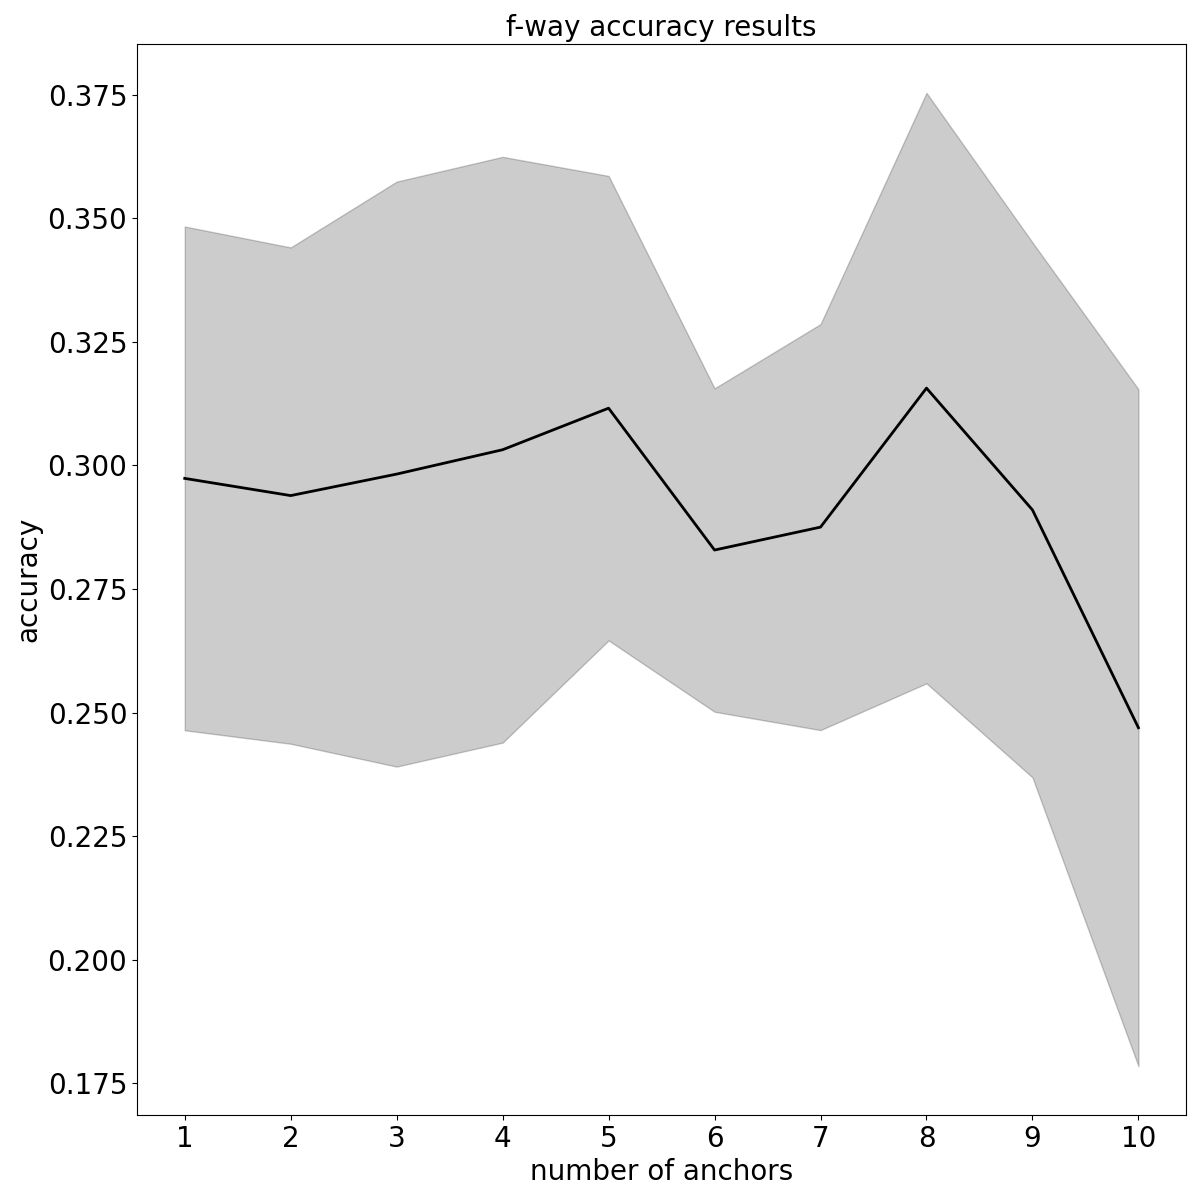
\includegraphics[width=0.65\textwidth]{./results/accuracy_trend_alohaMB.png}
        \vspace*{-0.2cm}
        \caption[ALOHA (M/B only) Family Prediction Accuracy Trend]{\textBF{Accuracy Trend} (varying the number of anchor samples used) resulting from the evaluation of the \textBF{ALOHA (M/B only)} implementation on the Malware Family Prediction task. The line represents the \textit{mean} Accuracy, while the shaded region represents the \textit{standard deviation}. Statistics were computed over 15 evaluation of the same model with different query and anchor samples.}
        \label{fig:alohaMBAccuracyTrend}
    \end{figure}
}

\newcommand{\jointEmbeddingAccuracyTrend}{
    \begin{figure}[H]
        \vspace*{-0.5cm}
        \centering
        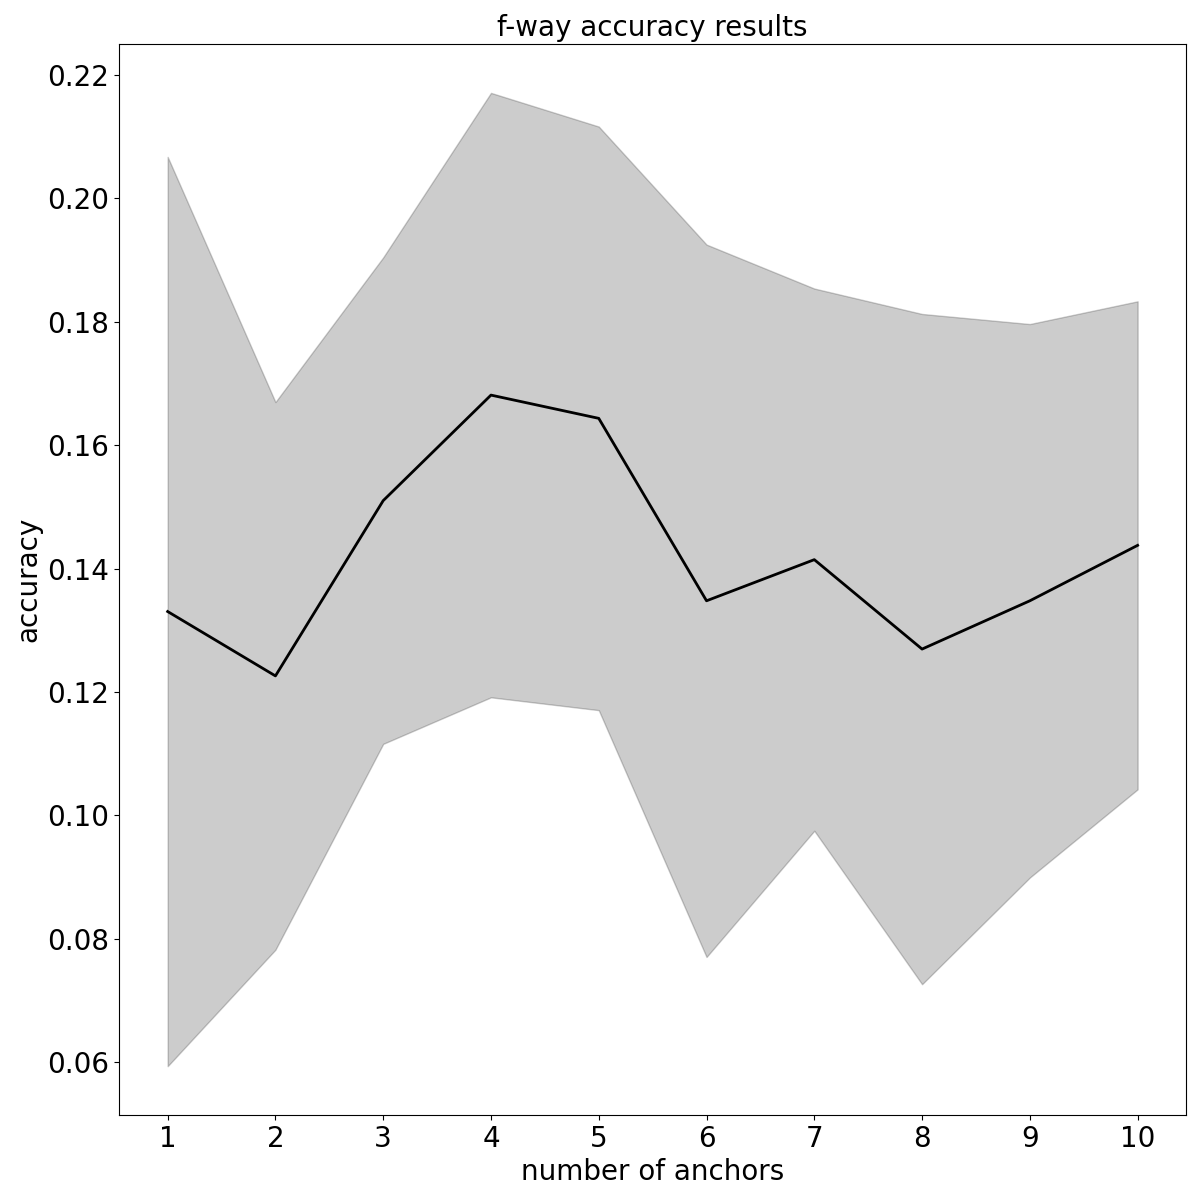
\includegraphics[width=0.65\textwidth]{./results/accuracy_trend_jointEmbedding.png}
        \vspace*{-0.2cm}
        \caption[Joint Embedding Family Prediction Accuracy Trend]{\textBF{Accuracy Trend} (varying the number of anchor samples used) resulting from the evaluation of the \textBF{Joint Embedding} implementation on the Malware Family Prediction task. The line represents the \textit{mean} Accuracy, while the shaded region represents the \textit{standard deviation}. Statistics were computed over 15 evaluation of the same model with different query and anchor samples.}
        \label{fig:jointEmbeddingAccuracyTrend}
    \end{figure}
}

\newcommand{\proposedModelAccuracyTrend}{
    \begin{figure}[H]
        \vspace*{-0.5cm}
        \centering
        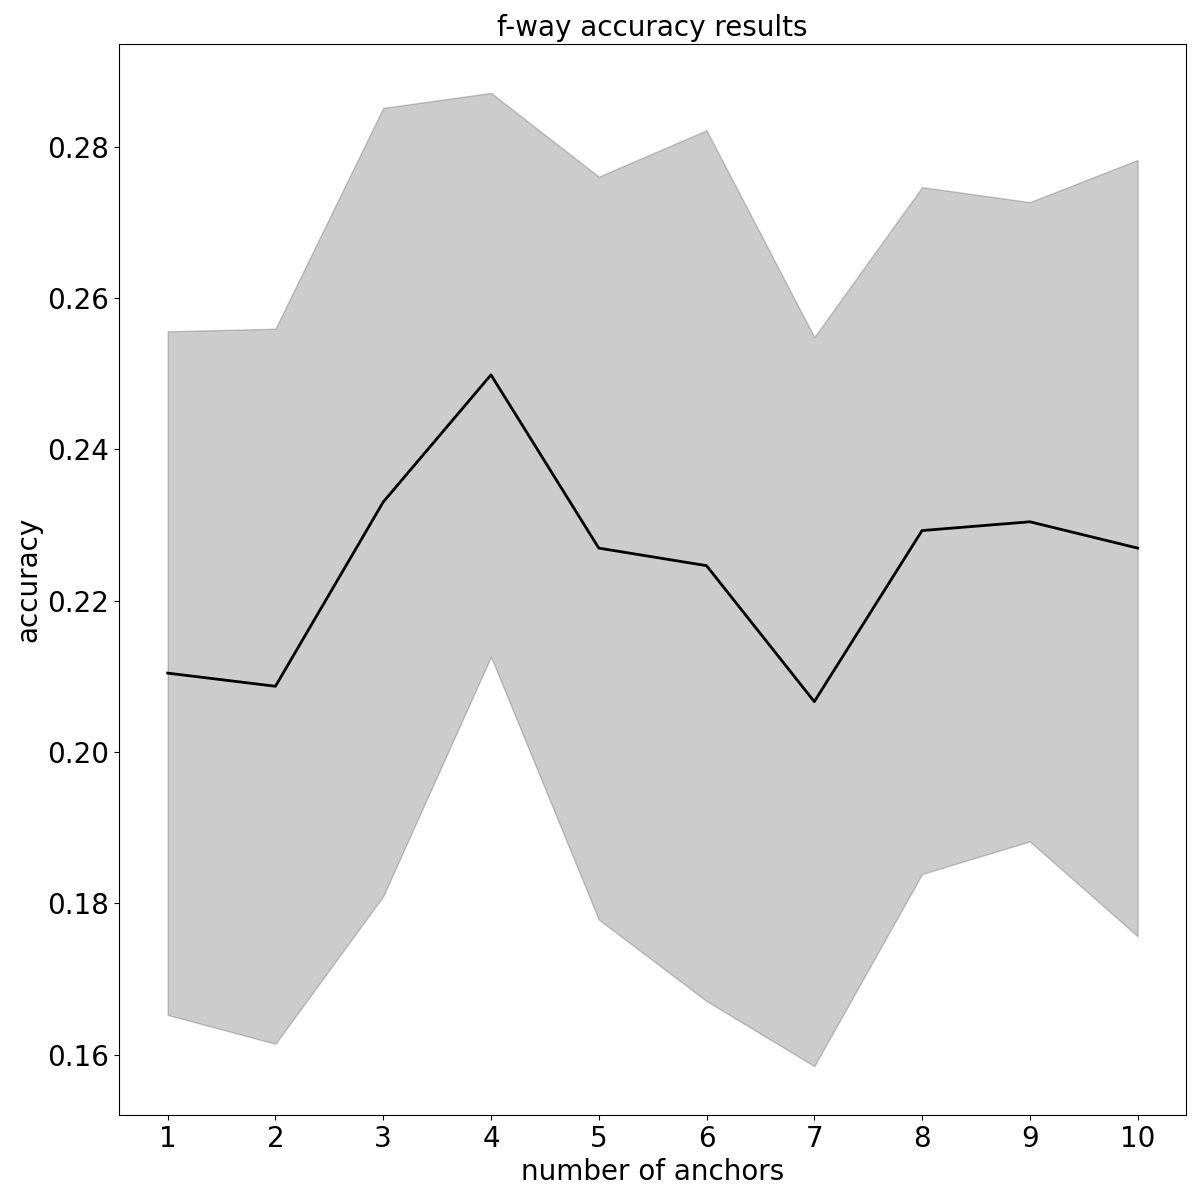
\includegraphics[width=0.65\textwidth]{./results/accuracy_trend_proposedModel.png}
        \vspace*{-0.2cm}
        \caption[Proposed Model Family Prediction Accuracy Trend]{\textBF{Accuracy Trend} (varying the number of anchor samples used) resulting from the evaluation of the \textBF{Proposed Model} implementation on the Malware Family Prediction task. The line represents the \textit{mean} Accuracy, while the shaded region represents the \textit{standard deviation}. Statistics were computed over 15 evaluation of the same model with different query and anchor samples.}
        \label{fig:proposedModelAccuracyTrend}
    \end{figure}
}

\newcommand{\alohaAucRocMacroTrend}{
    \begin{figure}[H]
        \vspace*{-0.5cm}
        \centering
        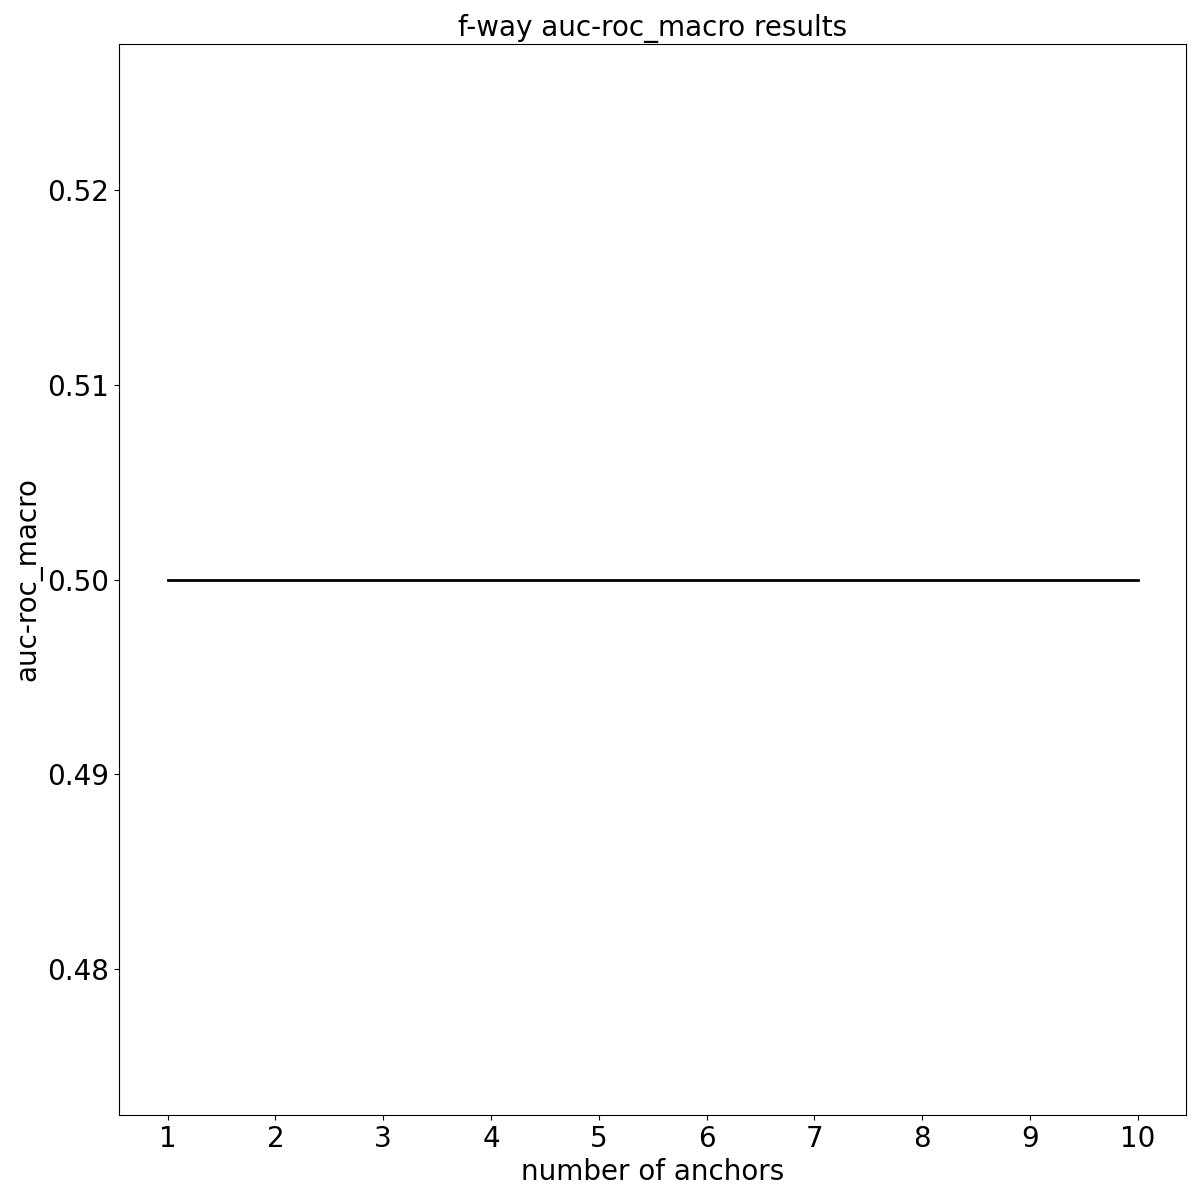
\includegraphics[width=0.65\textwidth]{./results/auc_roc_macro_trend_aloha.png}
        \vspace*{-0.2cm}
        \caption[ALOHA Family Prediction AUC-ROC Macro Trend]{\textBF{AUC-ROC Macro Trend} (varying the number of anchor samples used) resulting from the evaluation of the \textBF{ALOHA} implementation on the Malware Family Prediction task. The line represents the \textit{mean} Macro AUC-ROC, while the shaded region represents the \textit{standard deviation}. Statistics were computed over 15 evaluation of the same model with different query and anchor samples.}
        \label{fig:alohaAucRocMacroTrend}
    \end{figure}
}

\newcommand{\alohaMBAucRocMacroTrend}{
    \begin{figure}[H]
        \vspace*{-0.5cm}
        \centering
        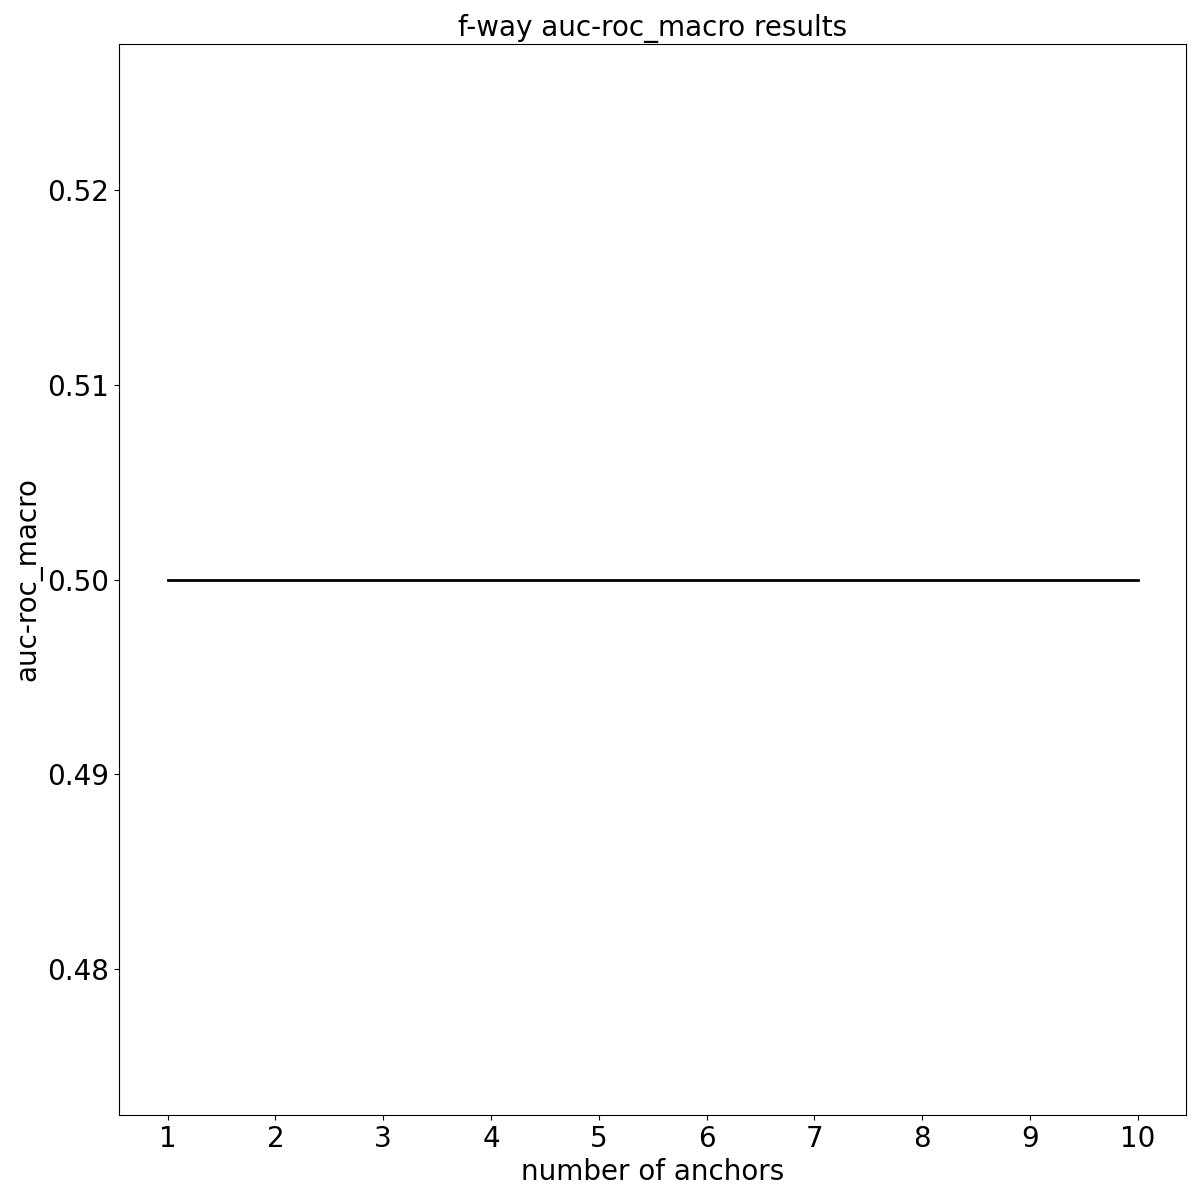
\includegraphics[width=0.65\textwidth]{./results/auc_roc_macro_trend_alohaMB.png}
        \vspace*{-0.2cm}
        \caption[ALOHA (M/B only) Family Prediction AUC-ROC Macro Trend]{\textBF{AUC-ROC Macro Trend} (varying the number of anchor samples used) resulting from the evaluation of the \textBF{ALOHA (M/B only)} implementation on the Malware Family Prediction task. The line represents the \textit{mean} Macro AUC-ROC, while the shaded region represents the \textit{standard deviation}. Statistics were computed over 15 evaluation of the same model with different query and anchor samples.}
        \label{fig:alohaMBAucRocMacroTrend}
    \end{figure}
}

\newcommand{\jointEmbeddingAucRocMacroTrend}{
    \begin{figure}[H]
        \vspace*{-0.5cm}
        \centering
        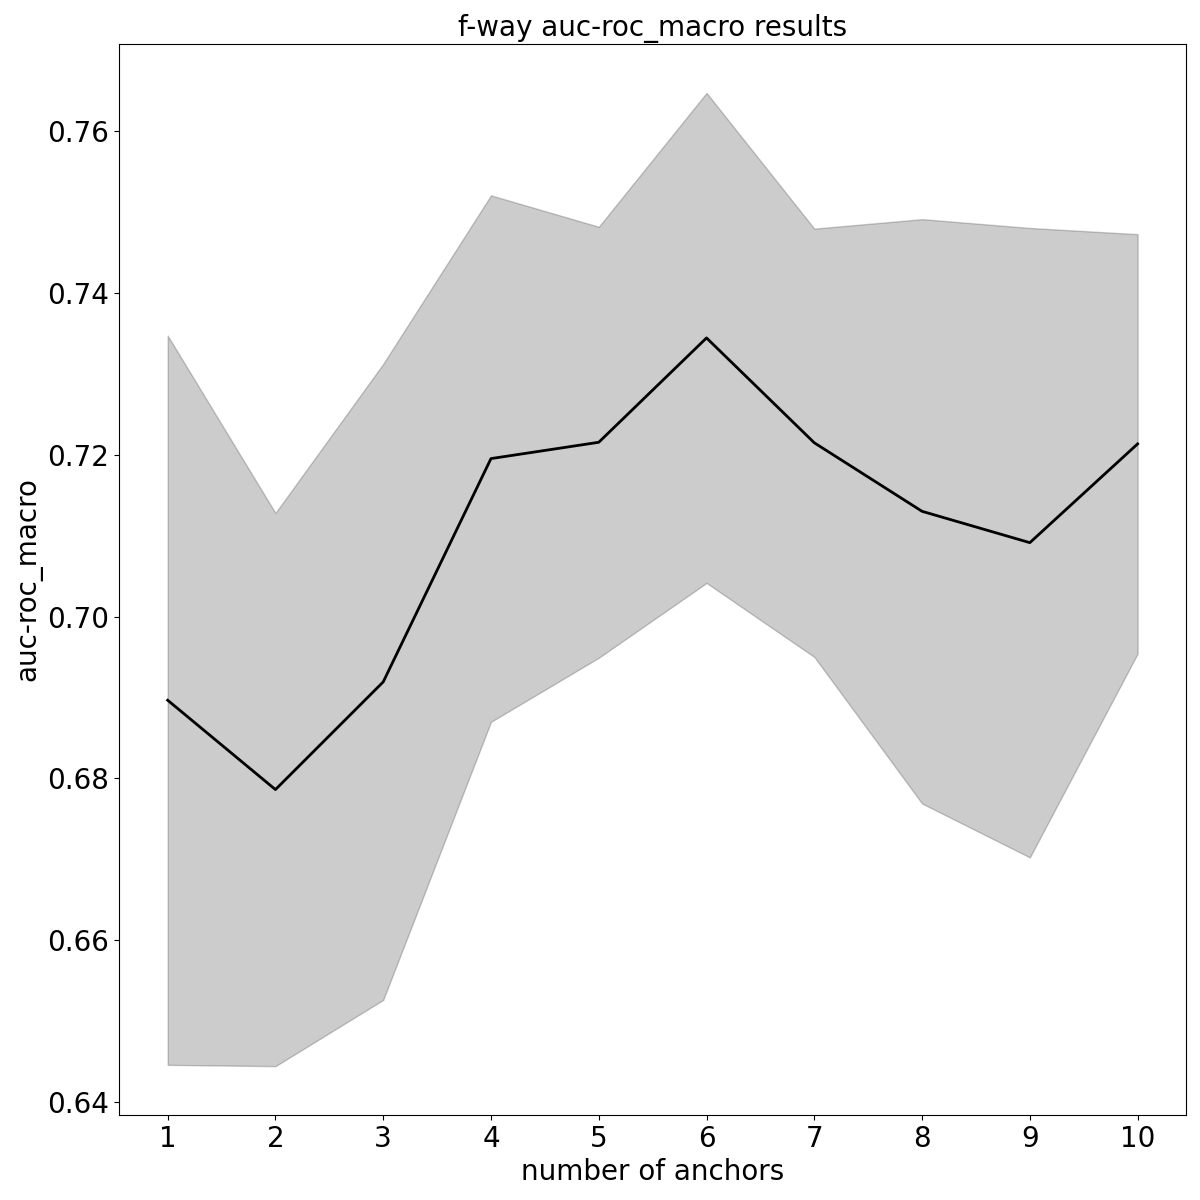
\includegraphics[width=0.65\textwidth]{./results/auc_roc_macro_trend_jointEmbedding.png}
        \vspace*{-0.2cm}
        \caption[Joint Embedding Family Prediction AUC-ROC Macro Trend]{\textBF{AUC-ROC Macro Trend} (varying the number of anchor samples used) resulting from the evaluation of the \textBF{Joint Embedding} implementation on the Malware Family Prediction task. The line represents the \textit{mean} Macro AUC-ROC, while the shaded region represents the \textit{standard deviation}. Statistics were computed over 15 evaluation of the same model with different query and anchor samples.}
        \label{fig:jointEmbeddingAucRocMacroTrend}
    \end{figure}
}

\newcommand{\proposedModelAucRocMacroTrend}{
    \begin{figure}[H]
        \vspace*{-0.5cm}
        \centering
        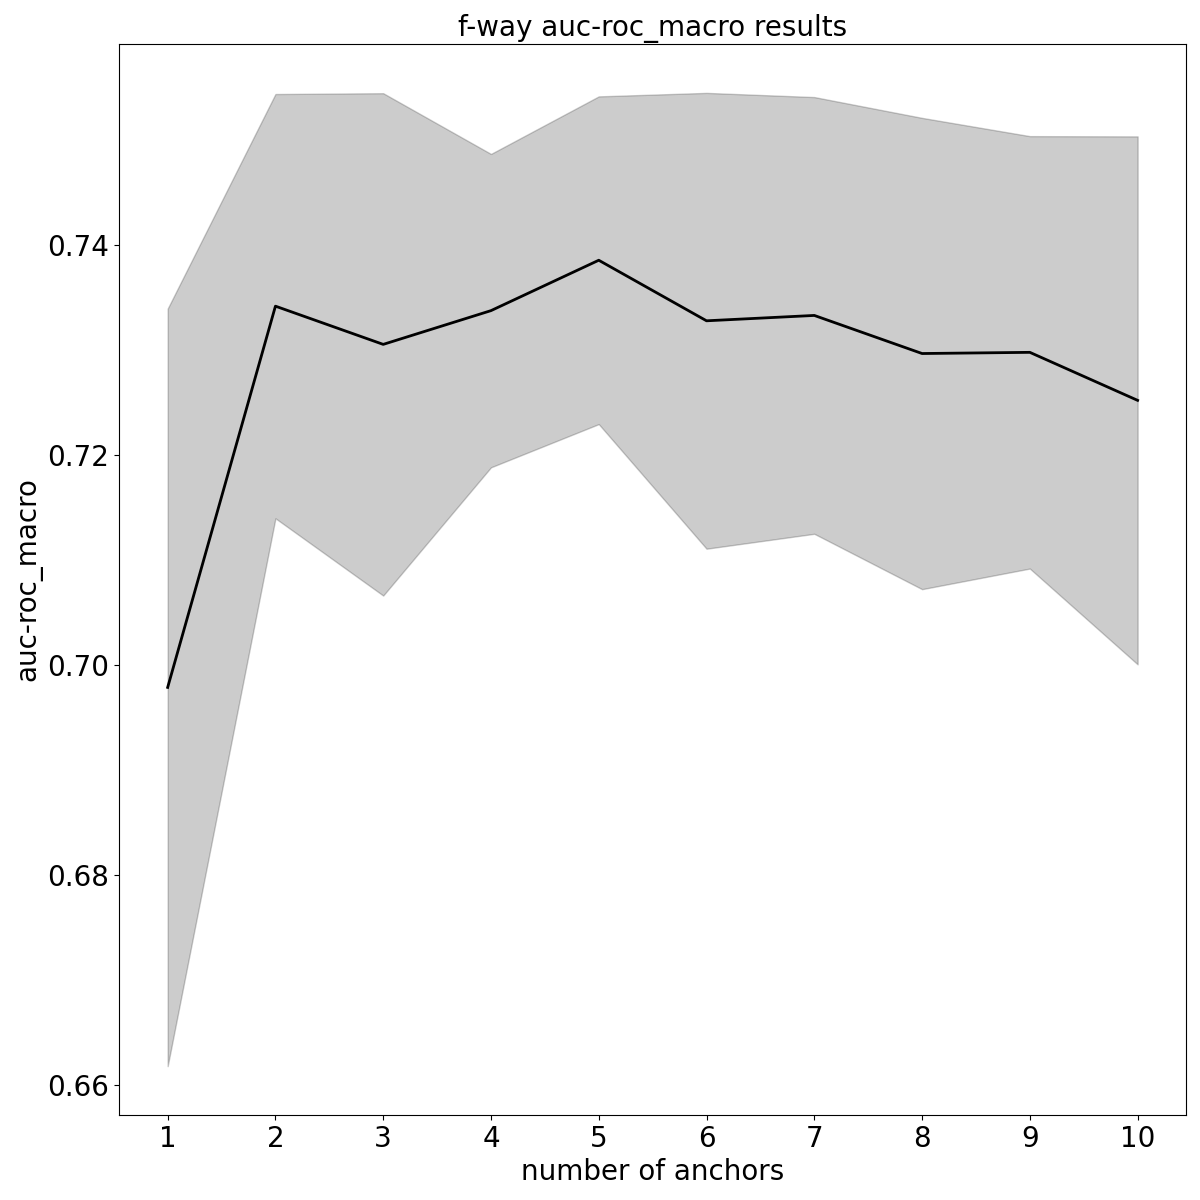
\includegraphics[width=0.65\textwidth]{./results/auc_roc_macro_trend_proposedModel.png}
        \vspace*{-0.2cm}
        \caption[Proposed Model Family Prediction AUC-ROC Macro Trend]{\textBF{AUC-ROC Macro Trend} (varying the number of anchor samples used) resulting from the evaluation of the \textBF{Proposed Model} implementation on the Malware Family Prediction task. The line represents the \textit{mean} Macro AUC-ROC, while the shaded region represents the \textit{standard deviation}. Statistics were computed over 15 evaluation of the same model with different query and anchor samples.}
        \label{fig:proposedModelAucRocMacroTrend}
    \end{figure}
}

\newcommand{\alohaAucRocMicroTrend}{
    \begin{figure}[H]
        \vspace*{-0.5cm}
        \centering
        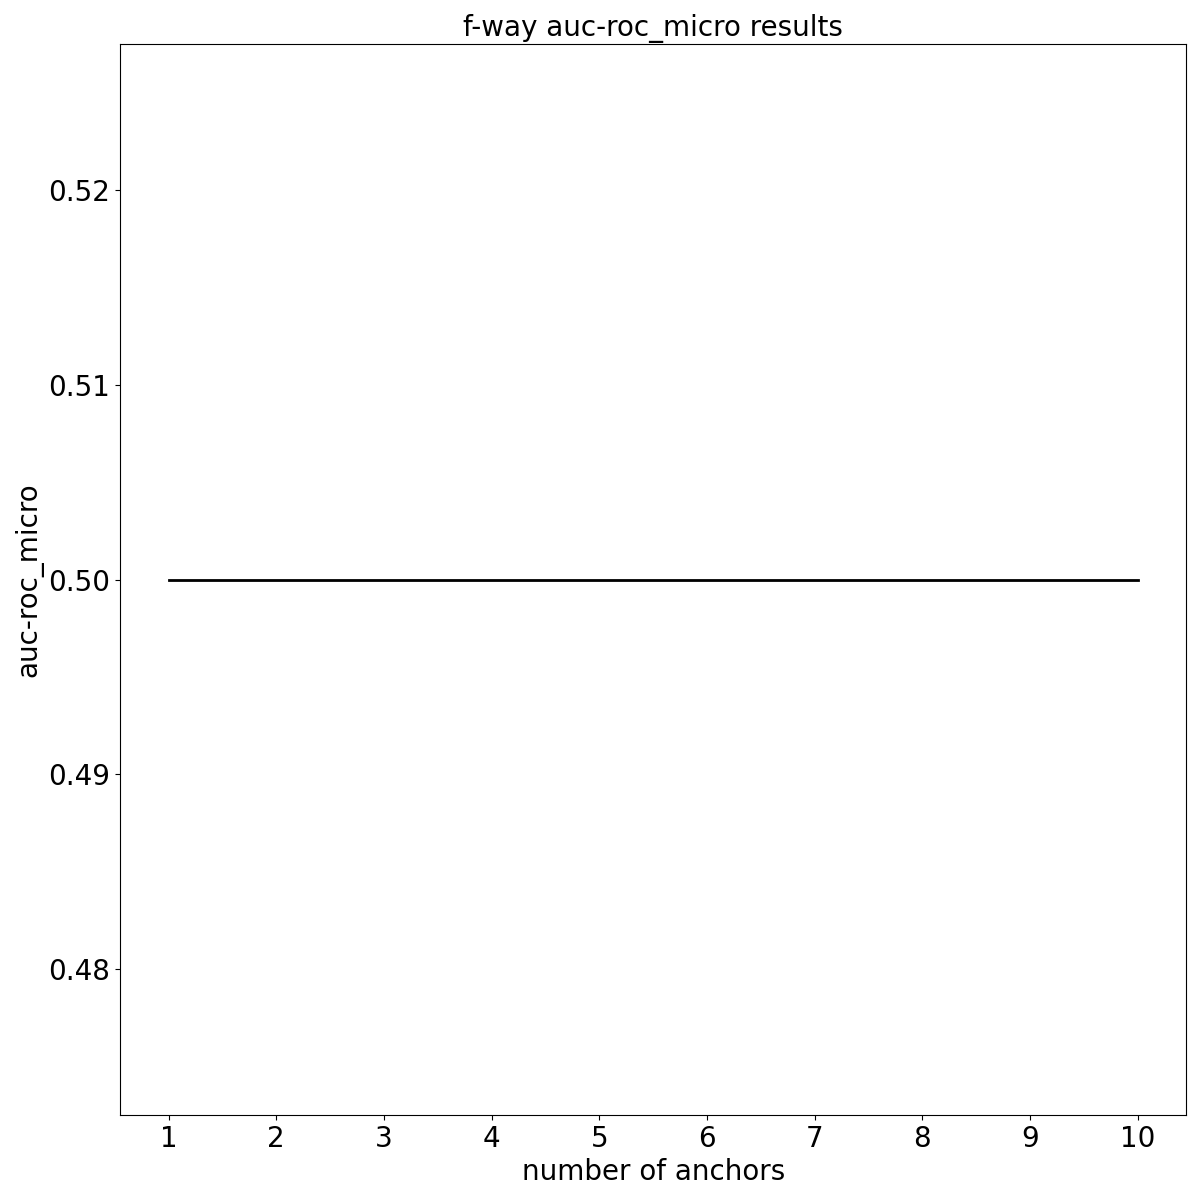
\includegraphics[width=0.65\textwidth]{./results/auc_roc_micro_trend_aloha.png}
        \vspace*{-0.2cm}
        \caption[ALOHA Family Prediction AUC-ROC Micro Trend]{\textBF{AUC-ROC Micro Trend} (varying the number of anchor samples used) resulting from the evaluation of the \textBF{ALOHA} implementation on the Malware Family Prediction task. The line represents the \textit{mean} Micro AUC-ROC, while the shaded region represents the \textit{standard deviation}. Statistics were computed over 15 evaluation of the same model with different query and anchor samples.}
        \label{fig:alohaAucRocMicroTrend}
    \end{figure}
}

\newcommand{\alohaMBAucRocMicroTrend}{
    \begin{figure}[H]
        \vspace*{-0.5cm}
        \centering
        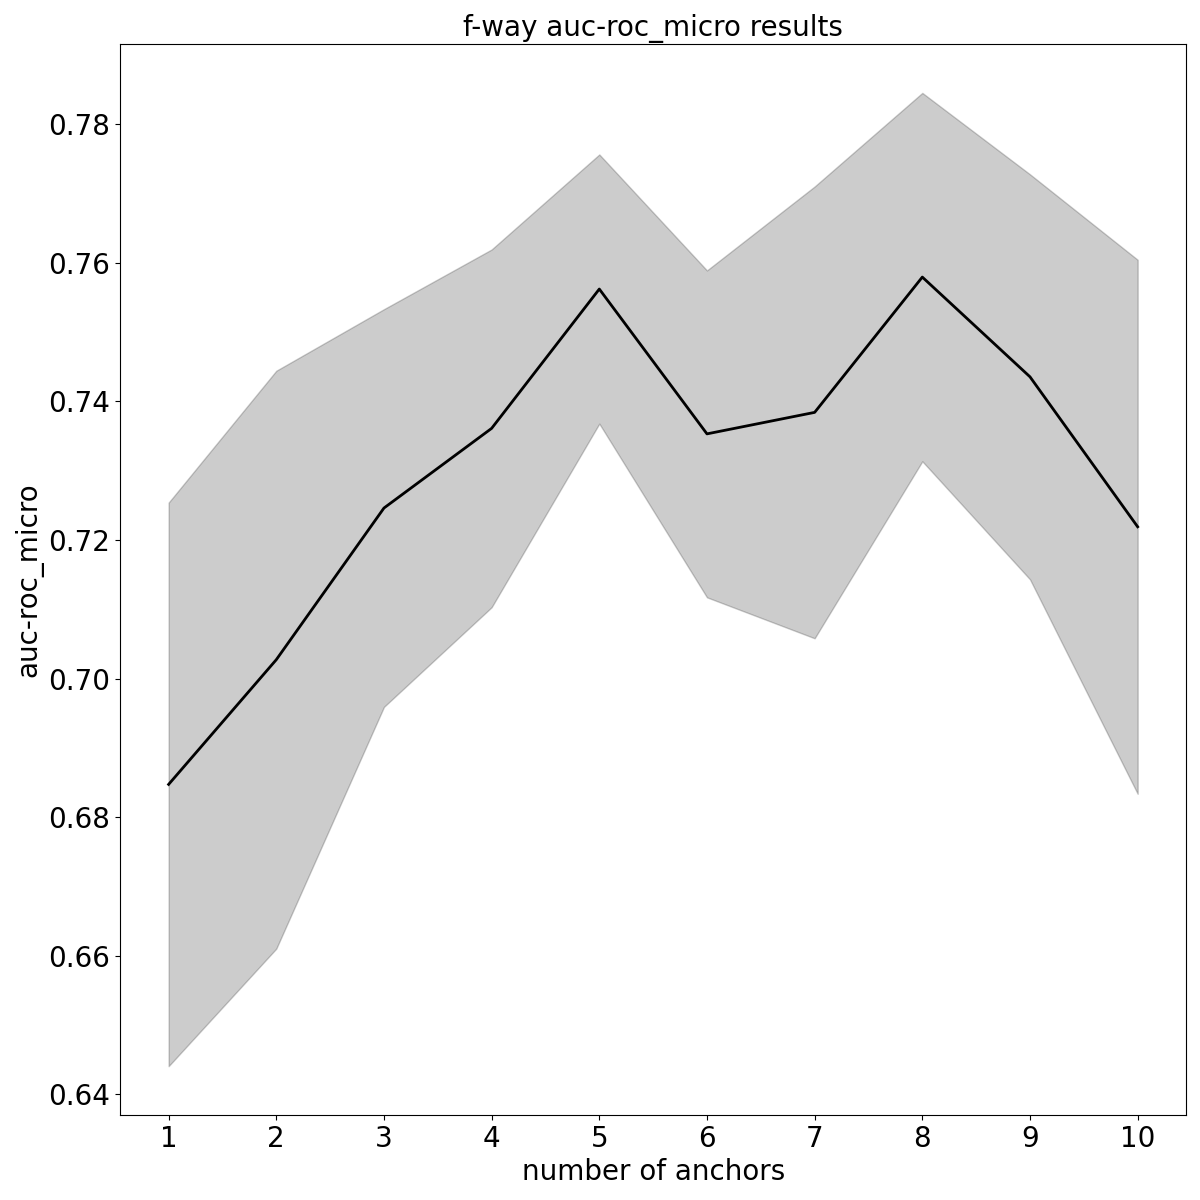
\includegraphics[width=0.65\textwidth]{./results/auc_roc_micro_trend_alohaMB.png}
        \vspace*{-0.2cm}
        \caption[ALOHA (M/B only) Family Prediction AUC-ROC Micro Trend]{\textBF{AUC-ROC Micro Trend} (varying the number of anchor samples used) resulting from the evaluation of the \textBF{ALOHA (M/B only)} implementation on the Malware Family Prediction task. The line represents the \textit{mean} Micro AUC-ROC, while the shaded region represents the \textit{standard deviation}. Statistics were computed over 15 evaluation of the same model with different query and anchor samples.}
        \label{fig:alohaMBAucRocMicroTrend}
    \end{figure}
}

\newcommand{\jointEmbeddingAucRocMicroTrend}{
    \begin{figure}[H]
        \vspace*{-0.5cm}
        \centering
        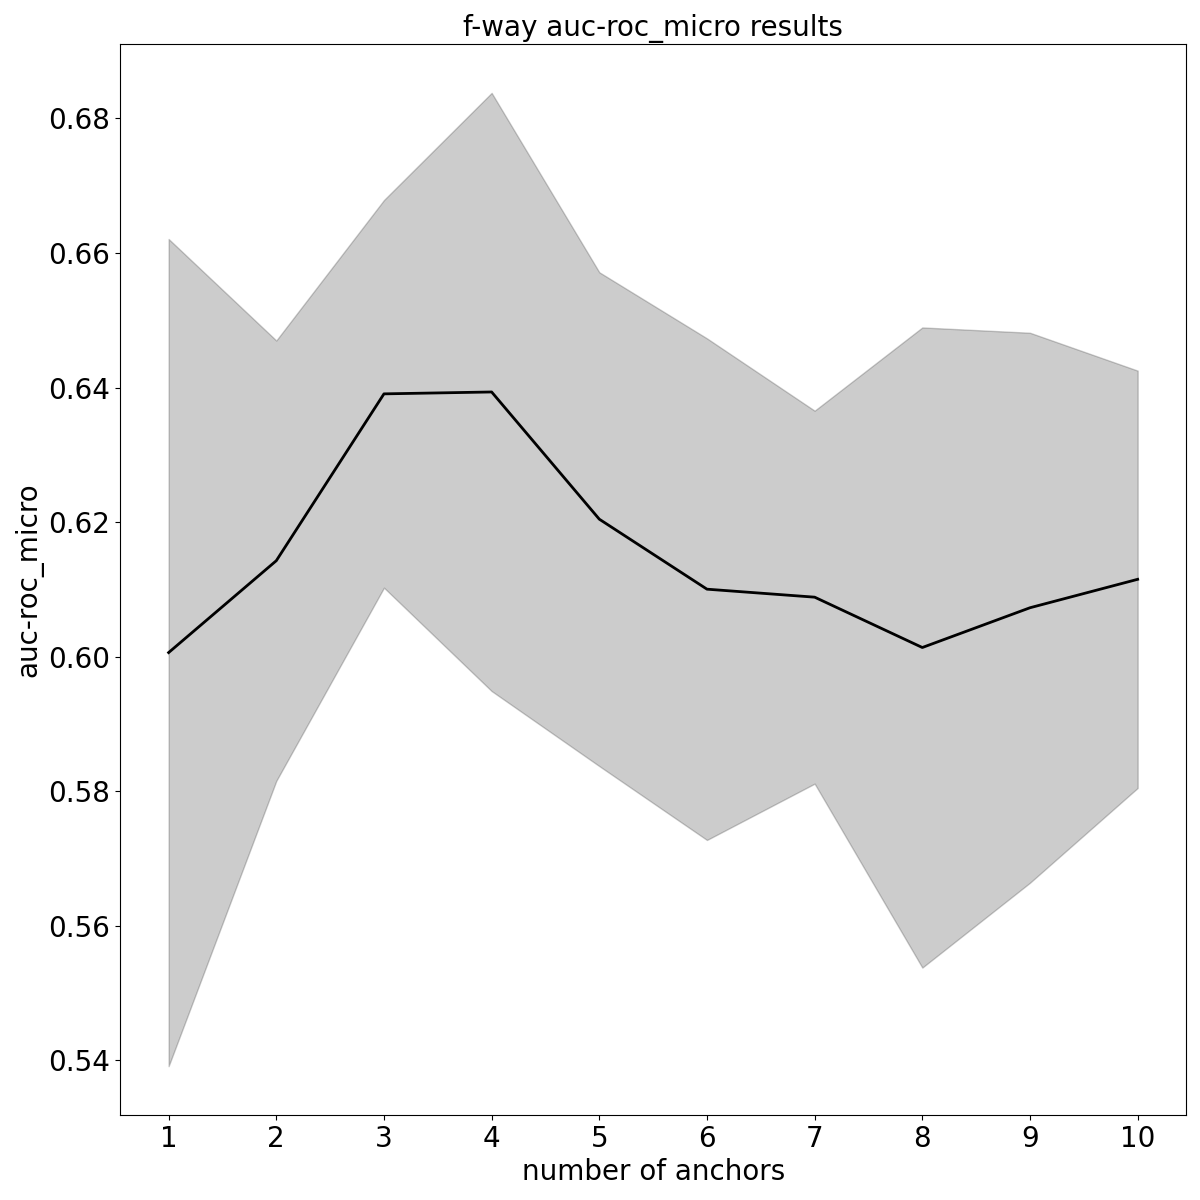
\includegraphics[width=0.65\textwidth]{./results/auc_roc_micro_trend_jointEmbedding.png}
        \vspace*{-0.2cm}
        \caption[Joint Embedding Family Prediction AUC-ROC Micro Trend]{\textBF{AUC-ROC Micro Trend} (varying the number of anchor samples used) resulting from the evaluation of the \textBF{Joint Embedding} implementation on the Malware Family Prediction task. The line represents the \textit{mean} Micro AUC-ROC, while the shaded region represents the \textit{standard deviation}. Statistics were computed over 15 evaluation of the same model with different query and anchor samples.}
        \label{fig:jointEmbeddingAucRocMicroTrend}
    \end{figure}
}

\newcommand{\proposedModelAucRocMicroTrend}{
    \begin{figure}[H]
        \vspace*{-0.5cm}
        \centering
        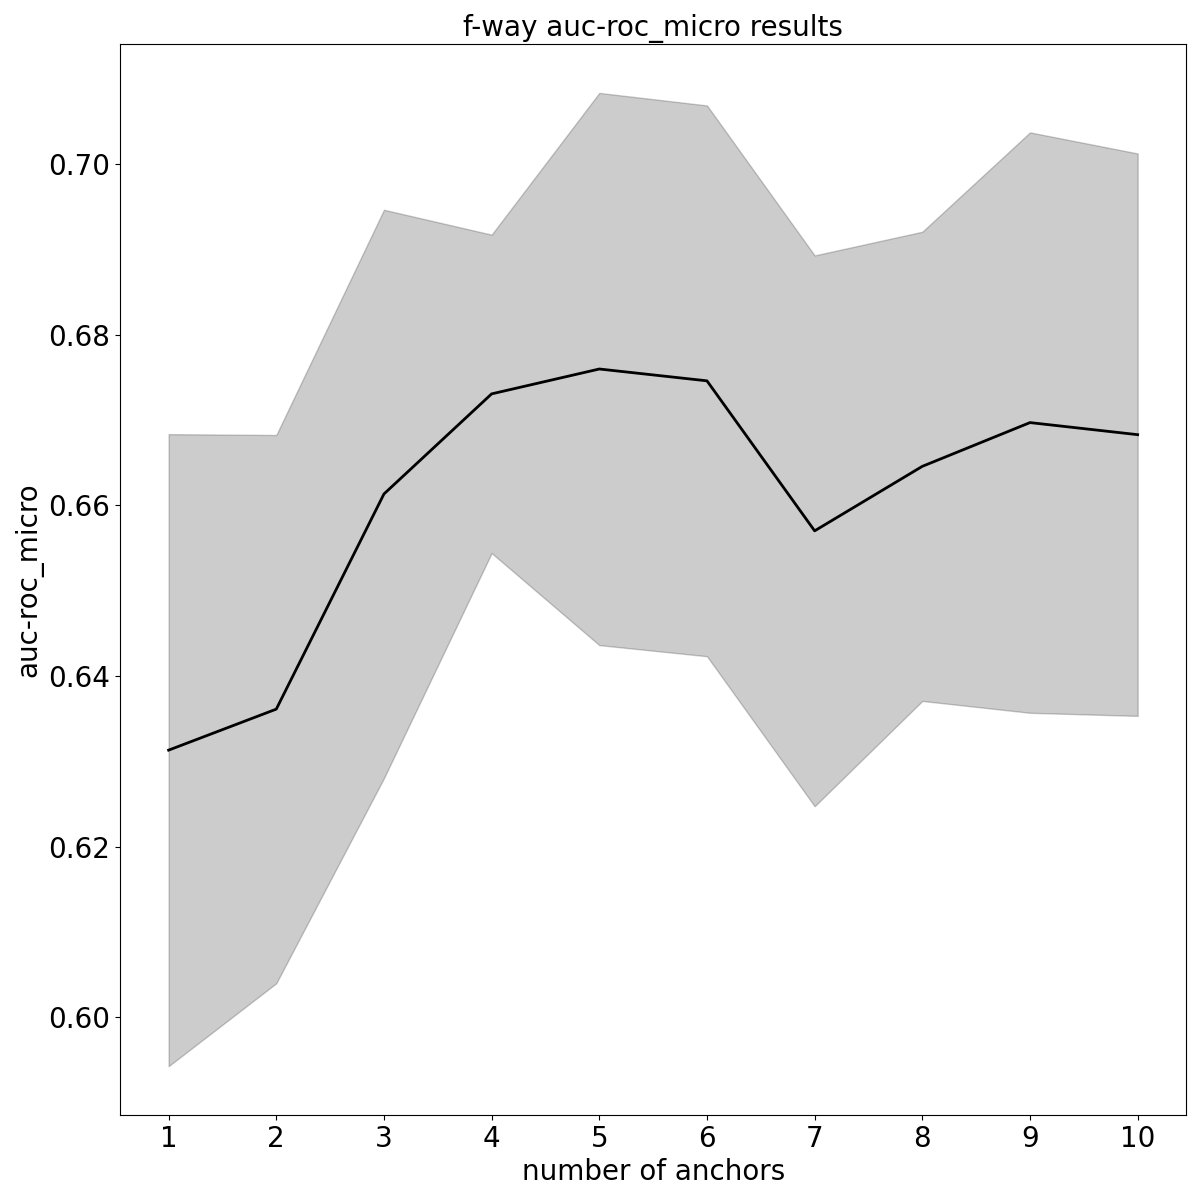
\includegraphics[width=0.65\textwidth]{./results/auc_roc_micro_trend_proposedModel.png}
        \vspace*{-0.2cm}
        \caption[Proposed Model Family Prediction AUC-ROC Micro Trend]{\textBF{AUC-ROC Micro Trend} (varying the number of anchor samples used) resulting from the evaluation of the \textBF{Proposed Model} implementation on the Malware Family Prediction task. The line represents the \textit{mean} Micro AUC-ROC, while the shaded region represents the \textit{standard deviation}. Statistics were computed over 15 evaluation of the same model with different query and anchor samples.}
        \label{fig:proposedModelAucRocMicroTrend}
    \end{figure}
}

\newcommand{\alohaFScoreMacroTrend}{
    \begin{figure}[H]
        \vspace*{-0.5cm}
        \centering
        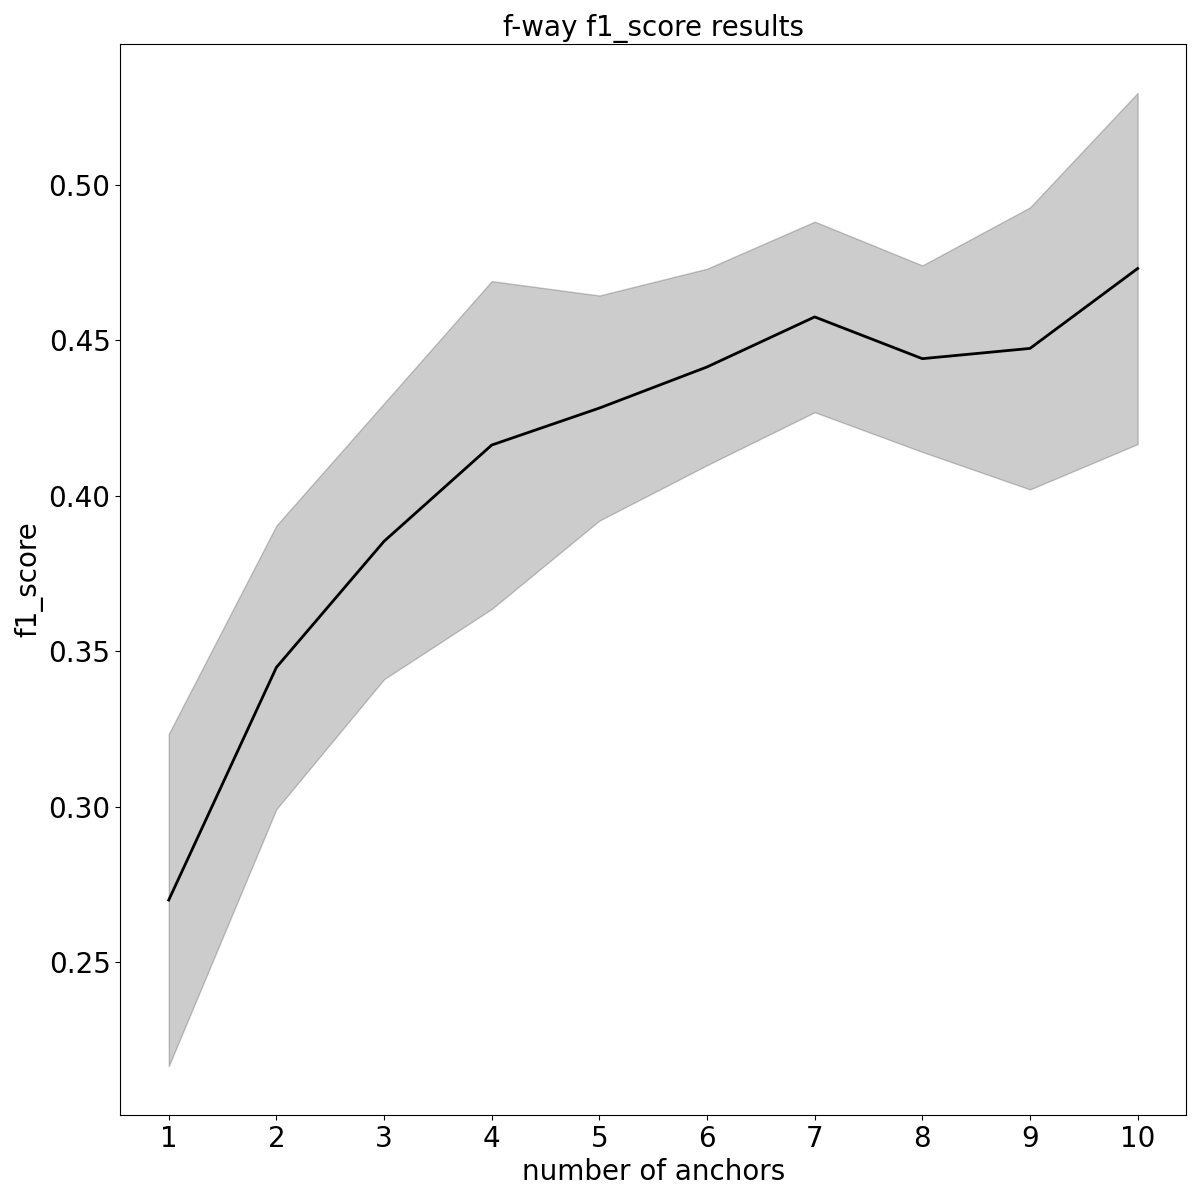
\includegraphics[width=0.65\textwidth]{./results/f1_score_macro_trend_aloha.png}
        \vspace*{-0.2cm}
        \caption[ALOHA Family Prediction F1-score Macro Trend]{\textBF{F1-score Macro Trend} (varying the number of anchor samples used) resulting from the evaluation of the \textBF{ALOHA} implementation on the Malware Family Prediction task. The line represents the \textit{mean} Macro F1-score, while the shaded region represents the \textit{standard deviation}. Statistics were computed over 15 evaluation of the same model with different query and anchor samples.}
        \label{fig:alohaF1ScoreMacroTrend}
    \end{figure}
}

\newcommand{\alohaMBFScoreMacroTrend}{
    \begin{figure}[H]
        \vspace*{-0.5cm}
        \centering
        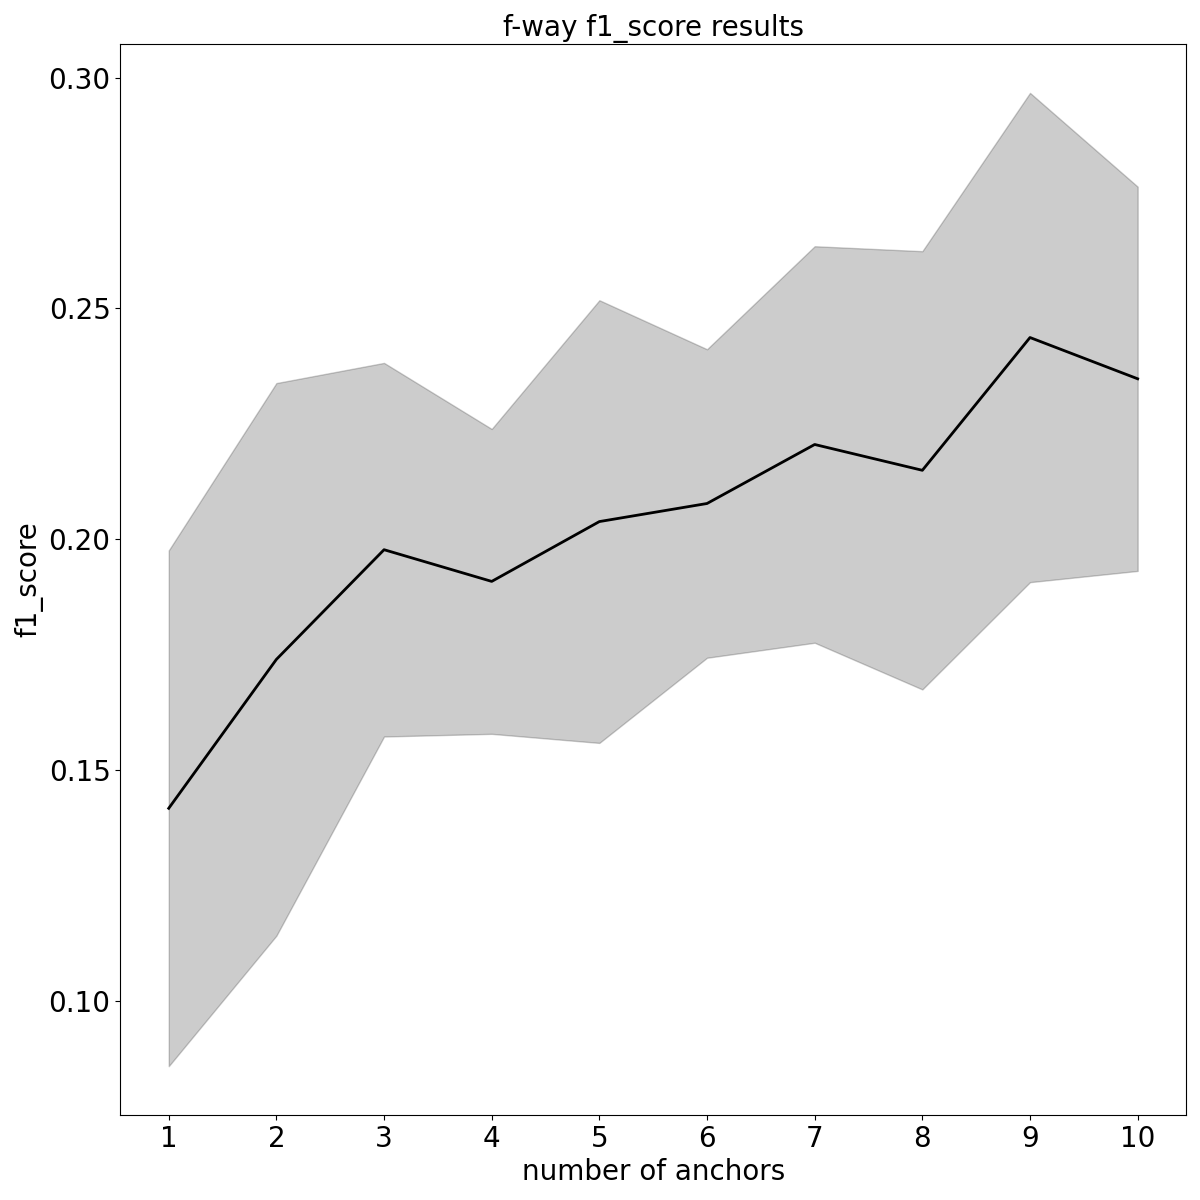
\includegraphics[width=0.65\textwidth]{./results/f1_score_macro_trend_alohaMB.png}
        \vspace*{-0.2cm}
        \caption[ALOHA (M/B only) Family Prediction F1-score Macro Trend]{\textBF{F1-score Macro Trend} (varying the number of anchor samples used) resulting from the evaluation of the \textBF{ALOHA (M/B only)} implementation on the Malware Family Prediction task. The line represents the \textit{mean} Macro F1-score, while the shaded region represents the \textit{standard deviation}. Statistics were computed over 15 evaluation of the same model with different query and anchor samples.}
        \label{fig:alohaMBF1ScoreMacroTrend}
    \end{figure}
}

\newcommand{\jointEmbeddingFScoreMacroTrend}{
    \begin{figure}[H]
        \vspace*{-0.5cm}
        \centering
        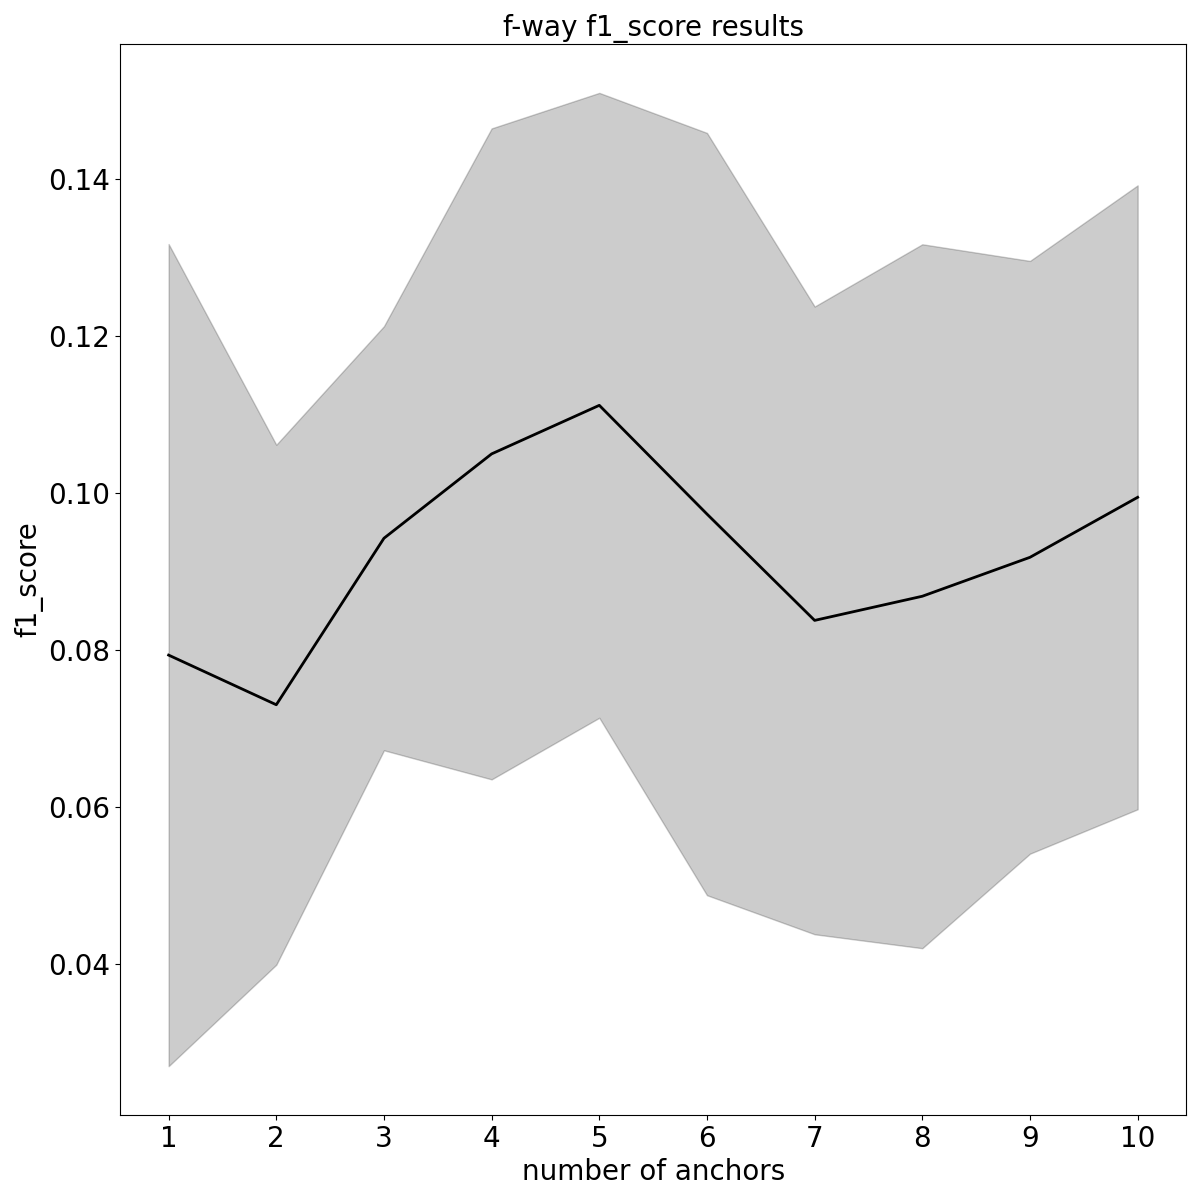
\includegraphics[width=0.65\textwidth]{./results/f1_score_macro_trend_jointEmbedding.png}
        \vspace*{-0.2cm}
        \caption[Joint Embedding Family Prediction F1-score Macro Trend]{\textBF{F1-score Macro Trend} (varying the number of anchor samples used) resulting from the evaluation of the \textBF{Joint Embedding} implementation on the Malware Family Prediction task. The line represents the \textit{mean} Macro F1-score, while the shaded region represents the \textit{standard deviation}. Statistics were computed over 15 evaluation of the same model with different query and anchor samples.}
        \label{fig:jointEmbeddingF1ScoreMacroTrend}
    \end{figure}
}

\newcommand{\proposedModelFScoreMacroTrend}{
    \begin{figure}[H]
        \vspace*{-0.5cm}
        \centering
        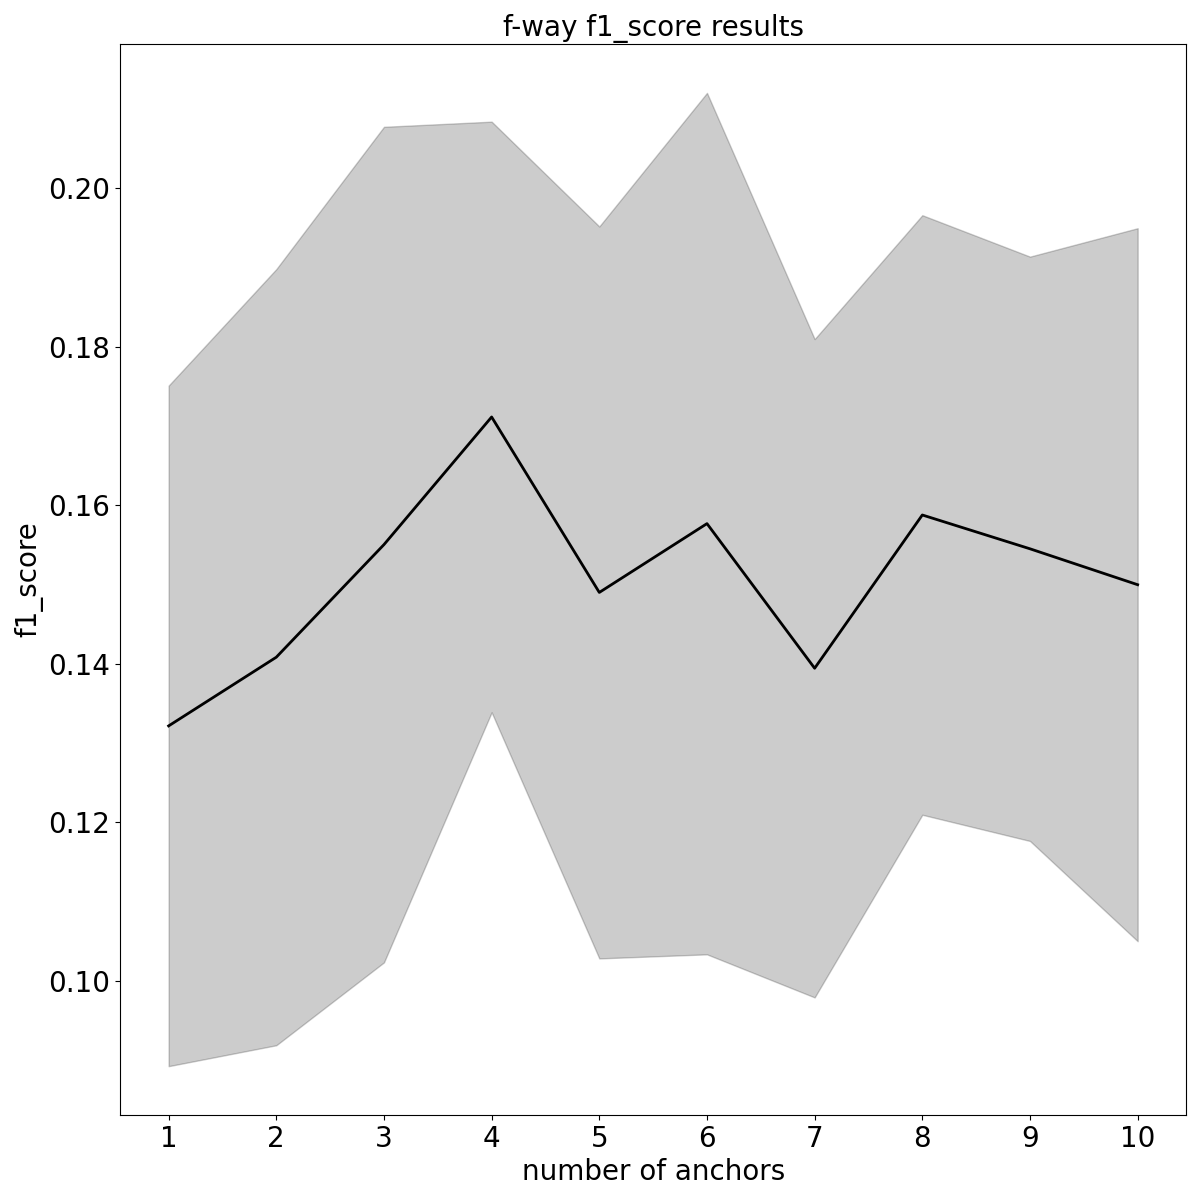
\includegraphics[width=0.65\textwidth]{./results/f1_score_macro_trend_proposedModel.png}
        \vspace*{-0.2cm}
        \caption[Proposed Model Family Prediction F1-score Macro Trend]{\textBF{F1-score Macro Trend} (varying the number of anchor samples used) resulting from the evaluation of the \textBF{Proposed Model} implementation on the Malware Family Prediction task. The line represents the \textit{mean} Macro F1-score, while the shaded region represents the \textit{standard deviation}. Statistics were computed over 15 evaluation of the same model with different query and anchor samples.}
        \label{fig:proposedModelF1ScoreMacroTrend}
    \end{figure}
}

\newcommand{\alohaFScoreMicroTrend}{
    \begin{figure}[H]
        \vspace*{-0.5cm}
        \centering
        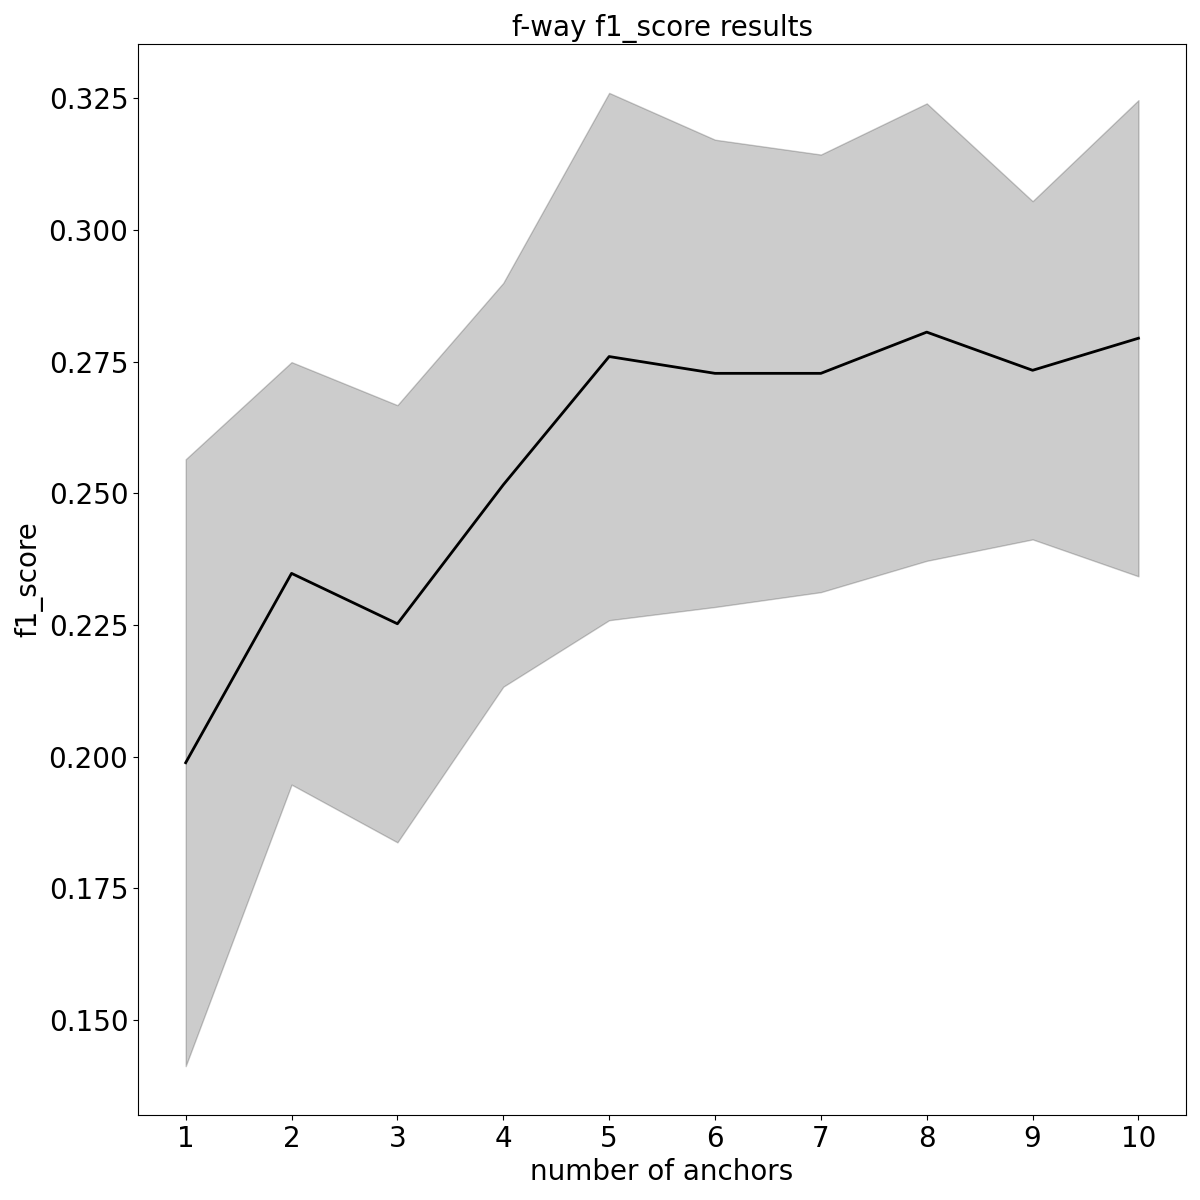
\includegraphics[width=0.65\textwidth]{./results/f1_score_micro_trend_aloha.png}
        \vspace*{-0.2cm}
        \caption[ALOHA Family Prediction F1-score Micro Trend]{\textBF{F1-score Micro Trend} (varying the number of anchor samples used) resulting from the evaluation of the \textBF{ALOHA} implementation on the Malware Family Prediction task. The line represents the \textit{mean} Micro F1-score, while the shaded region represents the \textit{standard deviation}. Statistics were computed over 15 evaluation of the same model with different query and anchor samples.}
        \label{fig:alohaF1ScoreMicroTrend}
    \end{figure}
}

\newcommand{\alohaMBFScoreMicroTrend}{
    \begin{figure}[H]
        \vspace*{-0.5cm}
        \centering
        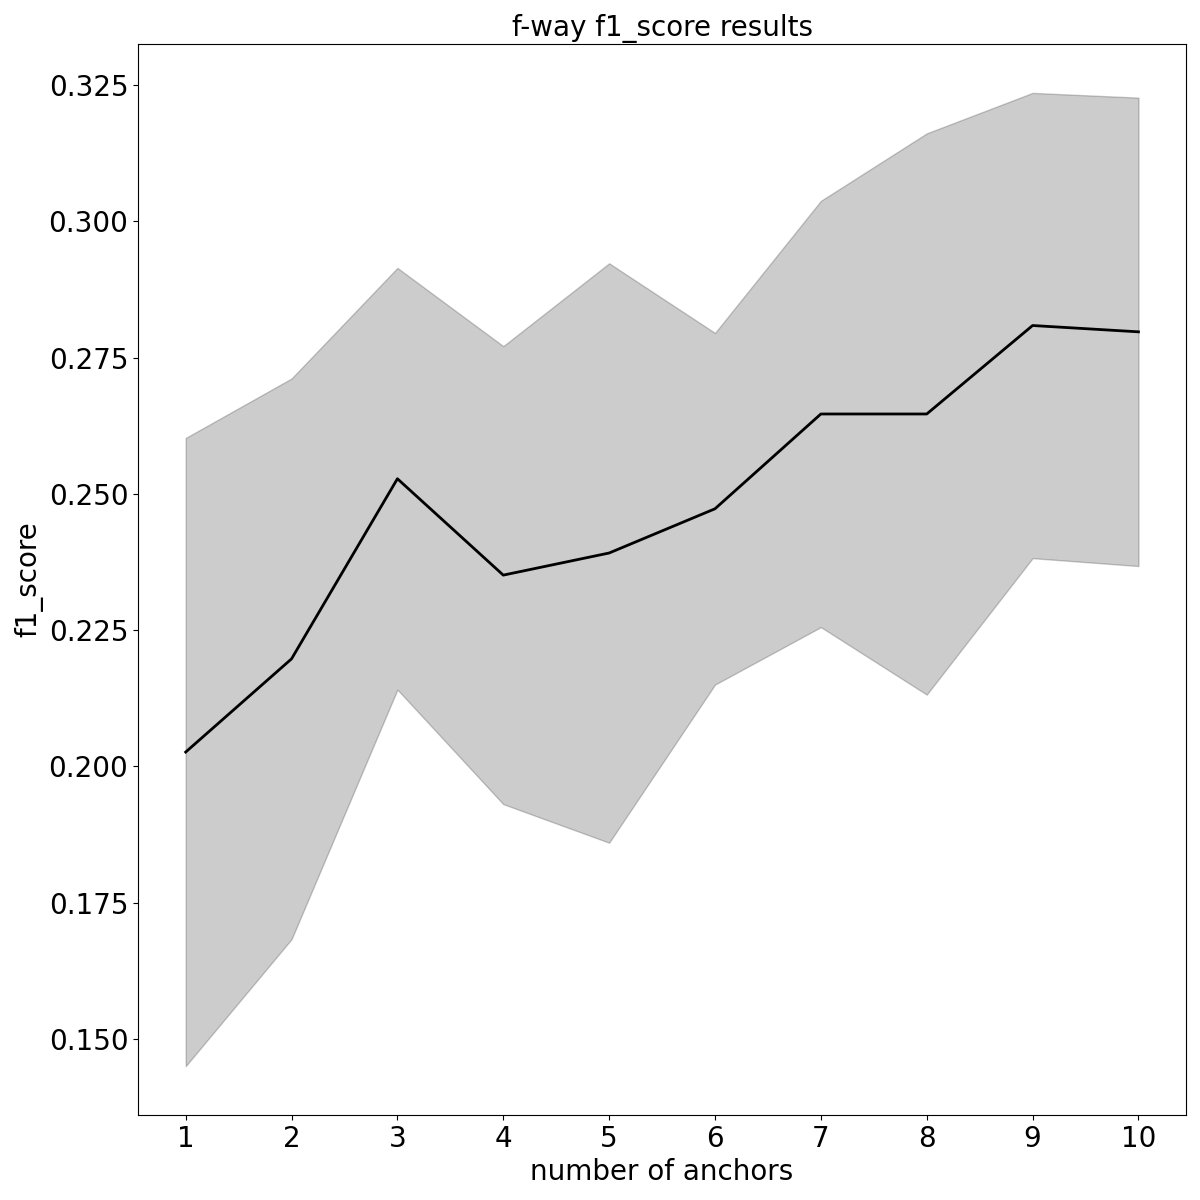
\includegraphics[width=0.65\textwidth]{./results/f1_score_micro_trend_alohaMB.png}
        \vspace*{-0.2cm}
        \caption[ALOHA (M/B only) Family Prediction F1-score Micro Trend]{\textBF{F1-score Micro Trend} (varying the number of anchor samples used) resulting from the evaluation of the \textBF{ALOHA (M/B only)} implementation on the Malware Family Prediction task. The line represents the \textit{mean} Micro F1-score, while the shaded region represents the \textit{standard deviation}. Statistics were computed over 15 evaluation of the same model with different query and anchor samples.}
        \label{fig:alohaMBF1ScoreMicroTrend}
    \end{figure}
}

\newcommand{\jointEmbeddingFScoreMicroTrend}{
    \begin{figure}[H]
        \vspace*{-0.5cm}
        \centering
        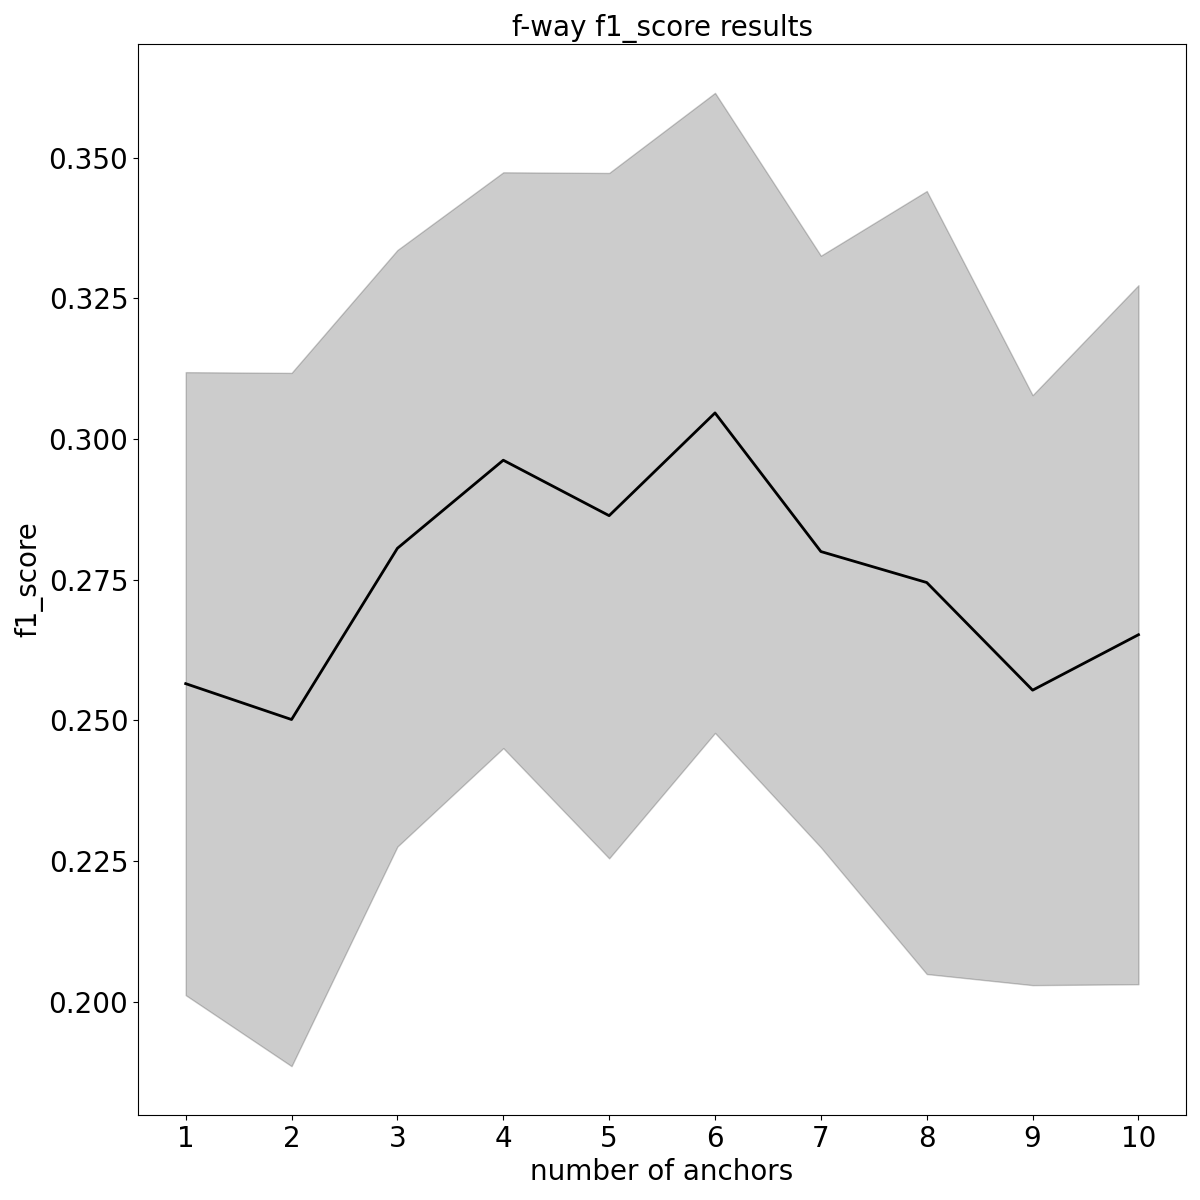
\includegraphics[width=0.65\textwidth]{./results/f1_score_micro_trend_jointEmbedding.png}
        \vspace*{-0.2cm}
        \caption[Joint Embedding Family Prediction F1-score Micro Trend]{\textBF{F1-score Micro Trend} (varying the number of anchor samples used) resulting from the evaluation of the \textBF{Joint Embedding} implementation on the Malware Family Prediction task. The line represents the \textit{mean} Micro F1-score, while the shaded region represents the \textit{standard deviation}. Statistics were computed over 15 evaluation of the same model with different query and anchor samples.}
        \label{fig:jointEmbeddingF1ScoreMicroTrend}
    \end{figure}
}

\newcommand{\proposedModelFScoreMicroTrend}{
    \begin{figure}[H]
        \vspace*{-0.5cm}
        \centering
        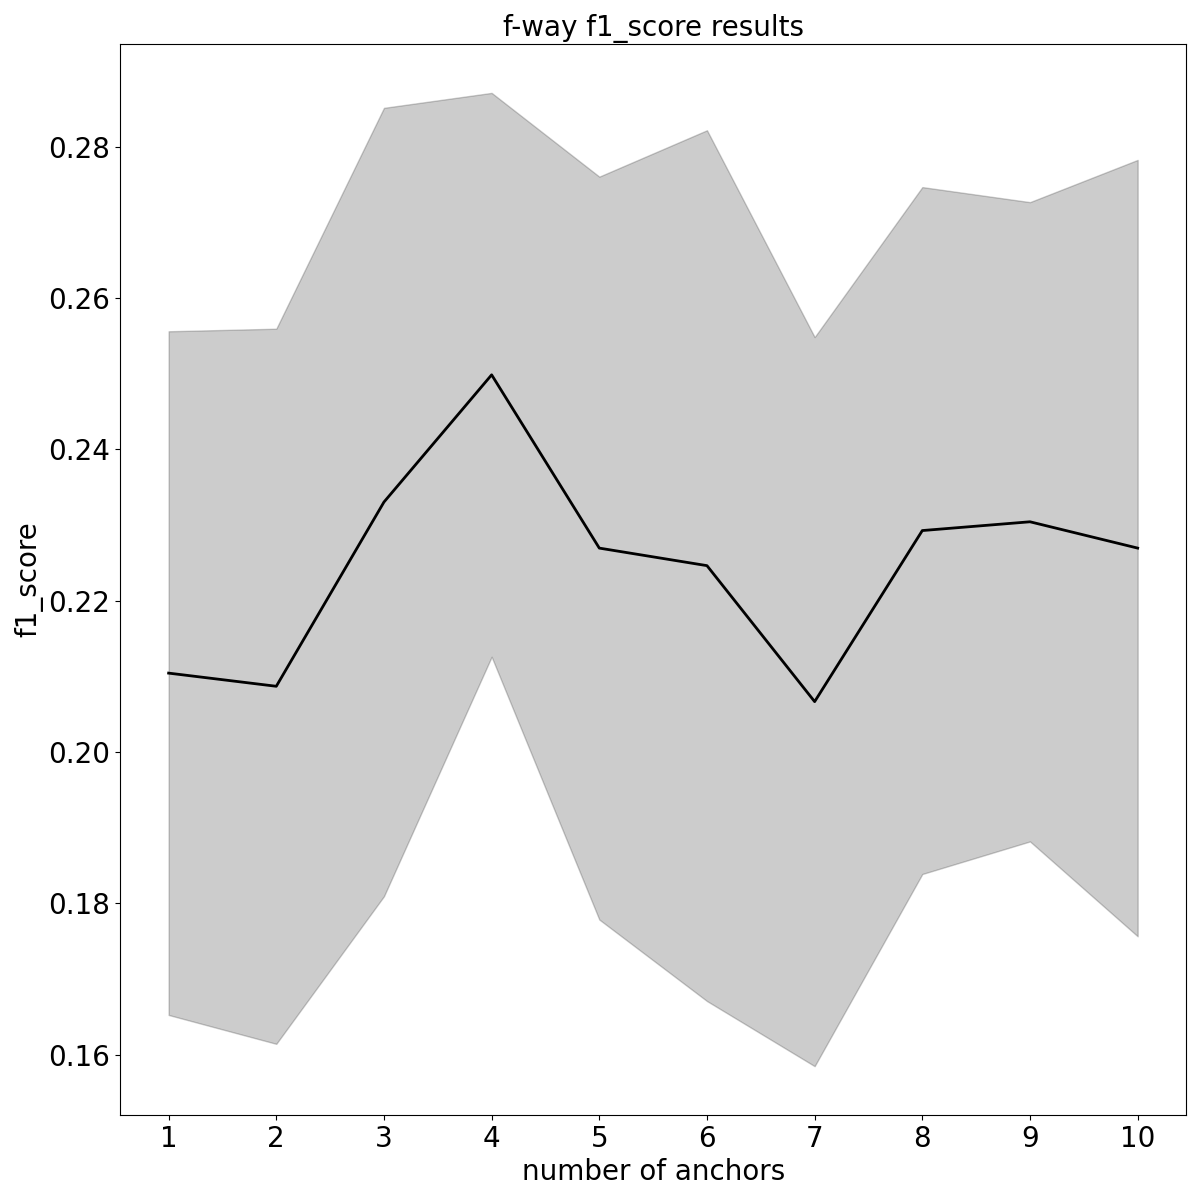
\includegraphics[width=0.65\textwidth]{./results/f1_score_micro_trend_proposedModel.png}
        \vspace*{-0.2cm}
        \caption[Proposed Model Family Prediction F1-score Micro Trend]{\textBF{F1-score Micro Trend} (varying the number of anchor samples used) resulting from the evaluation of the \textBF{Proposed Model} implementation on the Malware Family Prediction task. The line represents the \textit{mean} Micro F1-score, while the shaded region represents the \textit{standard deviation}. Statistics were computed over 15 evaluation of the same model with different query and anchor samples.}
        \label{fig:proposedModelF1ScoreMicroTrend}
    \end{figure}
}

\newcommand{\alohaPrecisionMacroTrend}{
    \begin{figure}[H]
        \vspace*{-0.5cm}
        \centering
        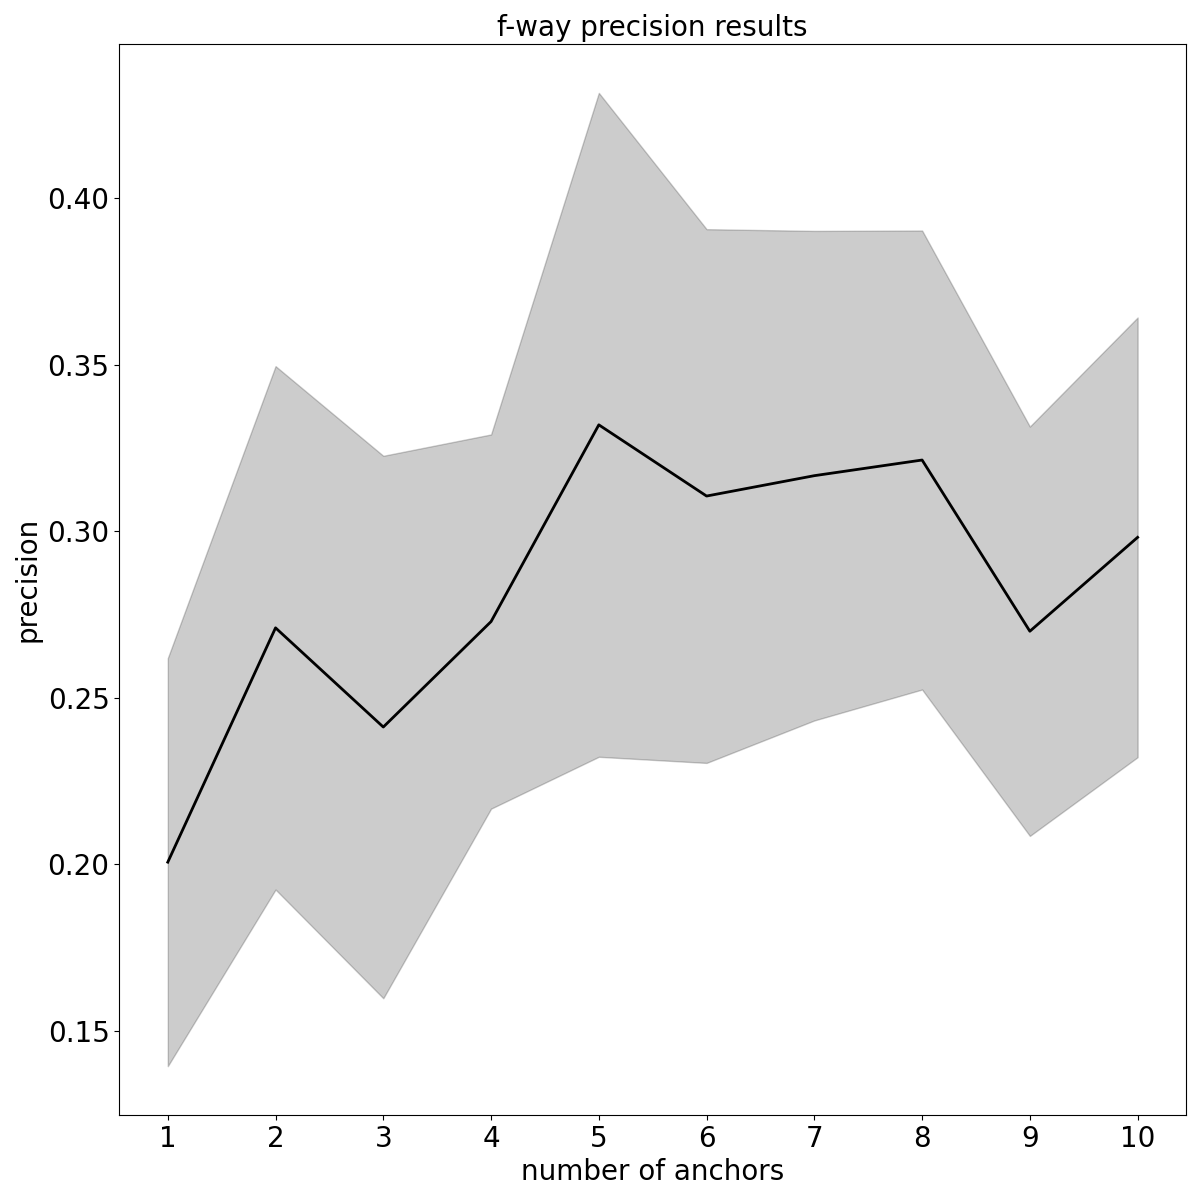
\includegraphics[width=0.65\textwidth]{./results/precision_macro_trend_aloha.png}
        \vspace*{-0.2cm}
        \caption[ALOHA Family Prediction Precision Macro Trend]{\textBF{Precision Macro Trend} (varying the number of anchor samples used) resulting from the evaluation of the \textBF{ALOHA} implementation on the Malware Family Prediction task. The line represents the \textit{mean} Macro Precision, while the shaded region represents the \textit{standard deviation}. Statistics were computed over 15 evaluation of the same model with different query and anchor samples.}
        \label{fig:alohaPrecisionMacroTrend}
    \end{figure}
}

\newcommand{\alohaMBPrecisionMacroTrend}{
    \begin{figure}[H]
        \vspace*{-0.5cm}
        \centering
        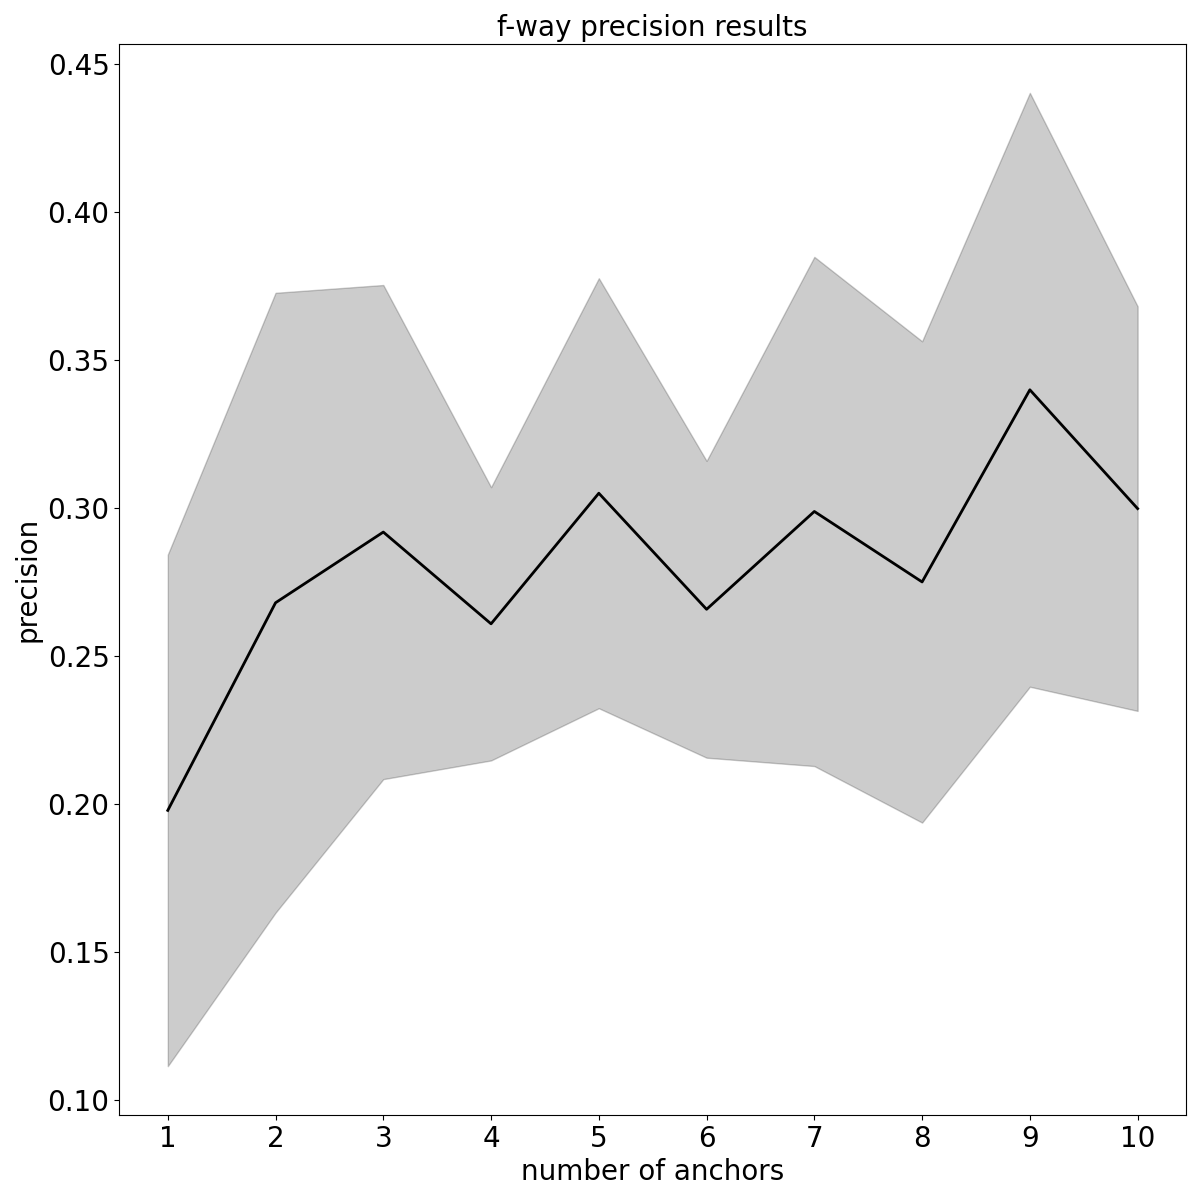
\includegraphics[width=0.65\textwidth]{./results/precision_macro_trend_alohaMB.png}
        \vspace*{-0.2cm}
        \caption[ALOHA (M/B only) Family Prediction Precision Macro Trend]{\textBF{Precision Macro Trend} (varying the number of anchor samples used) resulting from the evaluation of the \textBF{ALOHA (M/B only)} implementation on the Malware Family Prediction task. The line represents the \textit{mean} Macro Precision, while the shaded region represents the \textit{standard deviation}. Statistics were computed over 15 evaluation of the same model with different query and anchor samples.}
        \label{fig:alohaMBPrecisionMacroTrend}
    \end{figure}
}

\newcommand{\jointEmbeddingPrecisionMacroTrend}{
    \begin{figure}[H]
        \vspace*{-0.5cm}
        \centering
        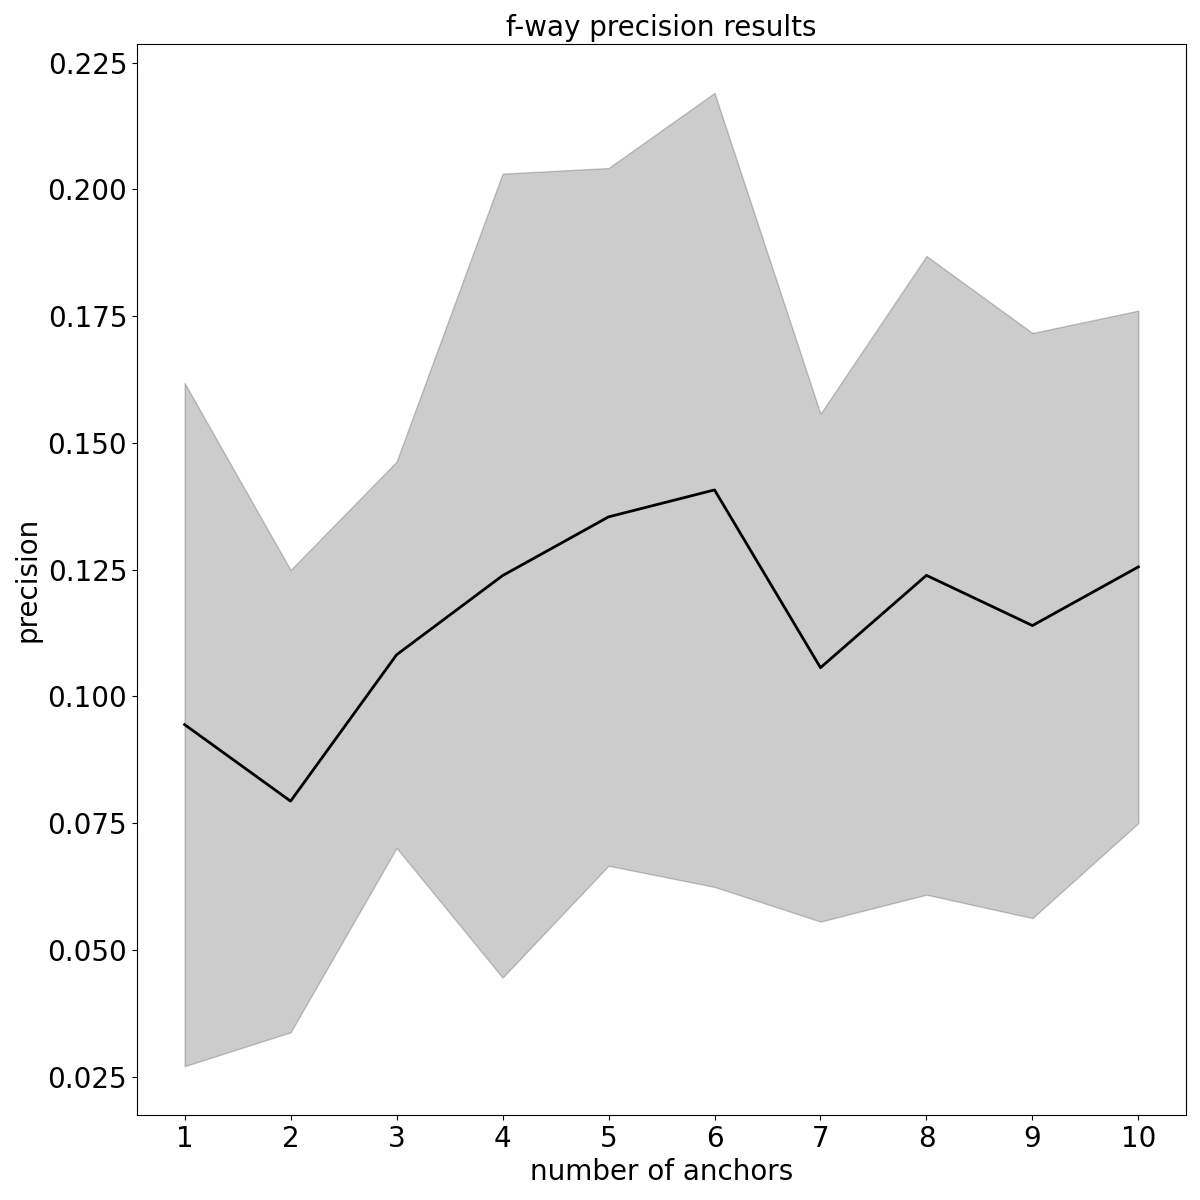
\includegraphics[width=0.65\textwidth]{./results/precision_macro_trend_jointEmbedding.png}
        \vspace*{-0.2cm}
        \caption[Joint Embedding Family Prediction Precision Macro Trend]{\textBF{Precision Macro Trend} (varying the number of anchor samples used) resulting from the evaluation of the \textBF{Joint Embedding} implementation on the Malware Family Prediction task. The line represents the \textit{mean} Macro Precision, while the shaded region represents the \textit{standard deviation}. Statistics were computed over 15 evaluation of the same model with different query and anchor samples.}
        \label{fig:jointEmbeddingPrecisionMacroTrend}
    \end{figure}
}

\newcommand{\proposedModelPrecisionMacroTrend}{
    \begin{figure}[H]
        \vspace*{-0.5cm}
        \centering
        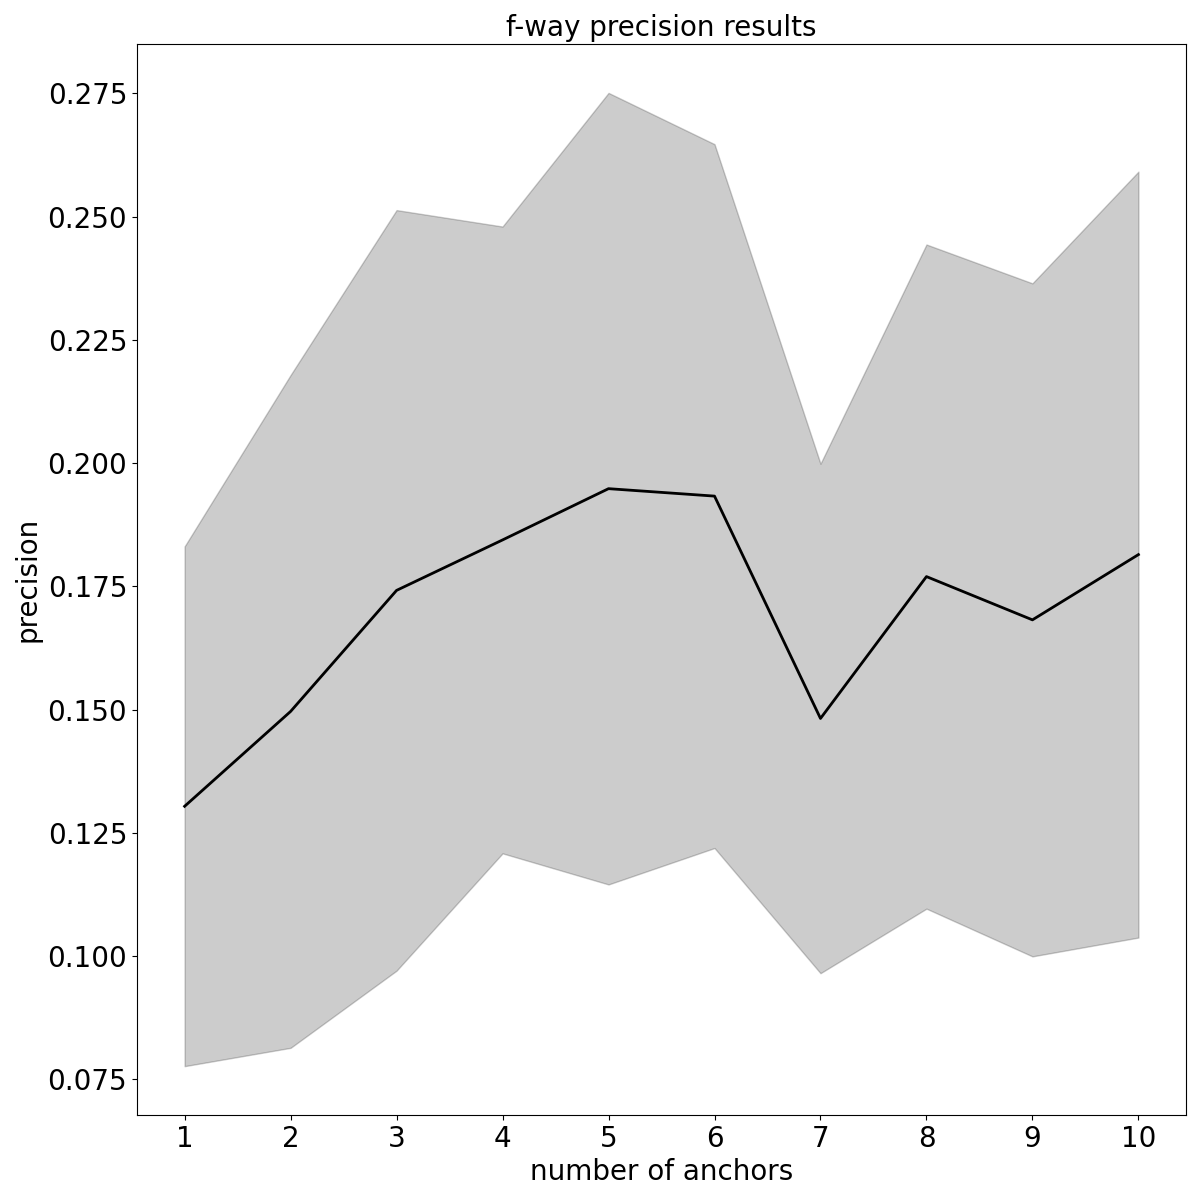
\includegraphics[width=0.65\textwidth]{./results/precision_macro_trend_proposedModel.png}
        \vspace*{-0.2cm}
        \caption[Proposed Model Family Prediction Precision Macro Trend]{\textBF{Precision Macro Trend} (varying the number of anchor samples used) resulting from the evaluation of the \textBF{Proposed Model} implementation on the Malware Family Prediction task. The line represents the \textit{mean} Macro Precision, while the shaded region represents the \textit{standard deviation}. Statistics were computed over 15 evaluation of the same model with different query and anchor samples.}
        \label{fig:proposedModelPrecisionMacroTrend}
    \end{figure}
}

\newcommand{\alohaPrecisionMicroTrend}{
    \begin{figure}[H]
        \vspace*{-0.5cm}
        \centering
        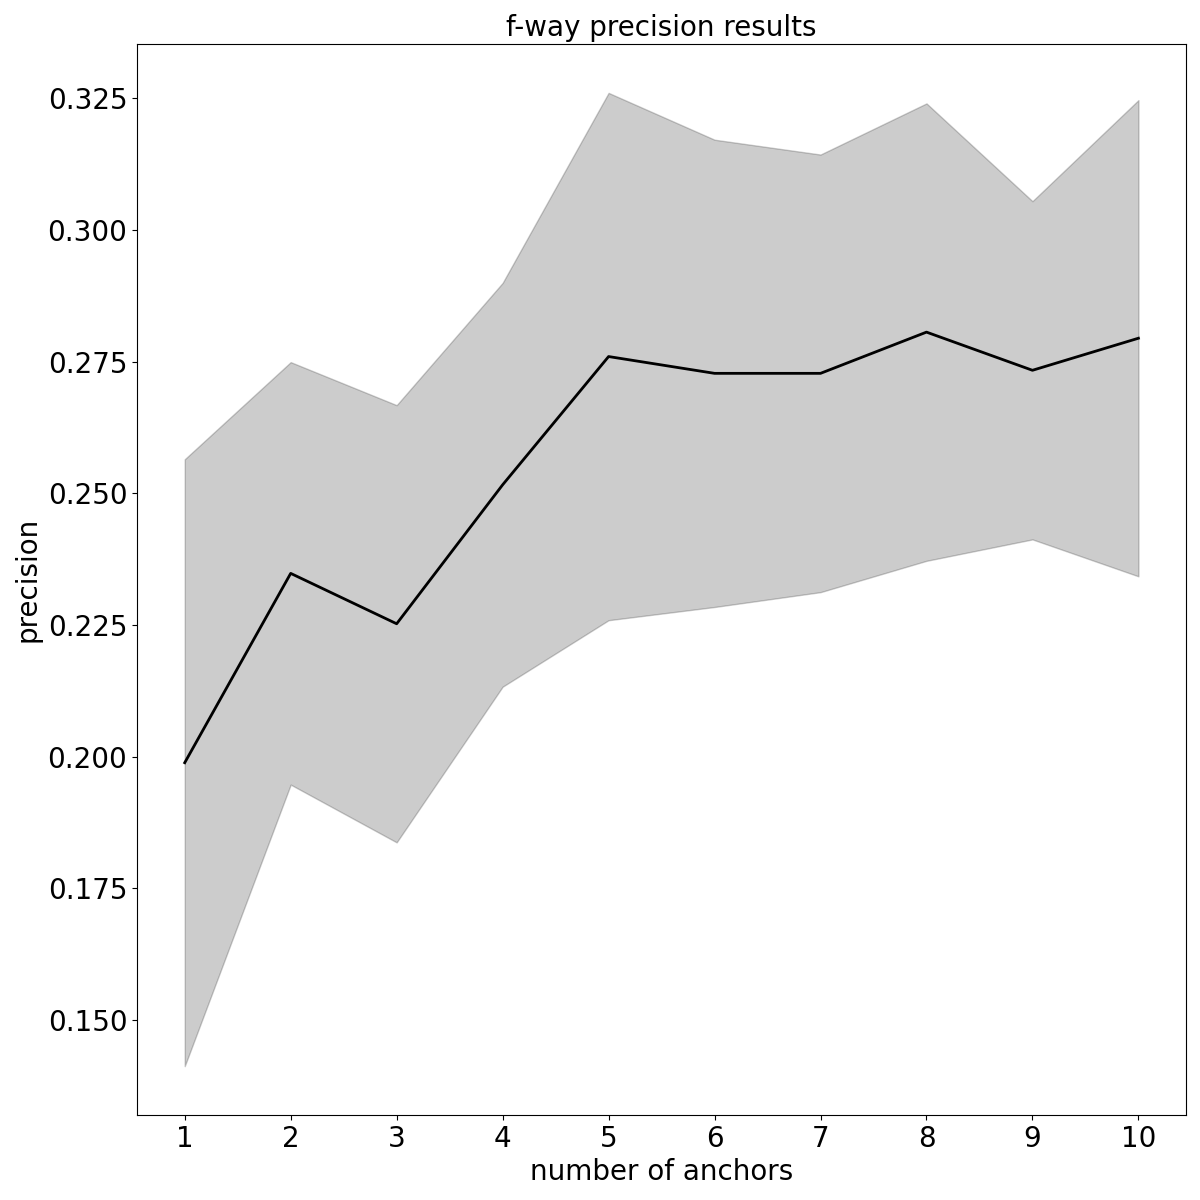
\includegraphics[width=0.65\textwidth]{./results/precision_micro_trend_aloha.png}
        \vspace*{-0.2cm}
        \caption[ALOHA Family Prediction Precision Micro Trend]{\textBF{Precision Micro Trend} (varying the number of anchor samples used) resulting from the evaluation of the \textBF{ALOHA} implementation on the Malware Family Prediction task. The line represents the \textit{mean} Micro Precision, while the shaded region represents the \textit{standard deviation}. Statistics were computed over 15 evaluation of the same model with different query and anchor samples.}
        \label{fig:alohaPrecisionMicroTrend}
    \end{figure}
}

\newcommand{\alohaMBPrecisionMicroTrend}{
    \begin{figure}[H]
        \vspace*{-0.5cm}
        \centering
        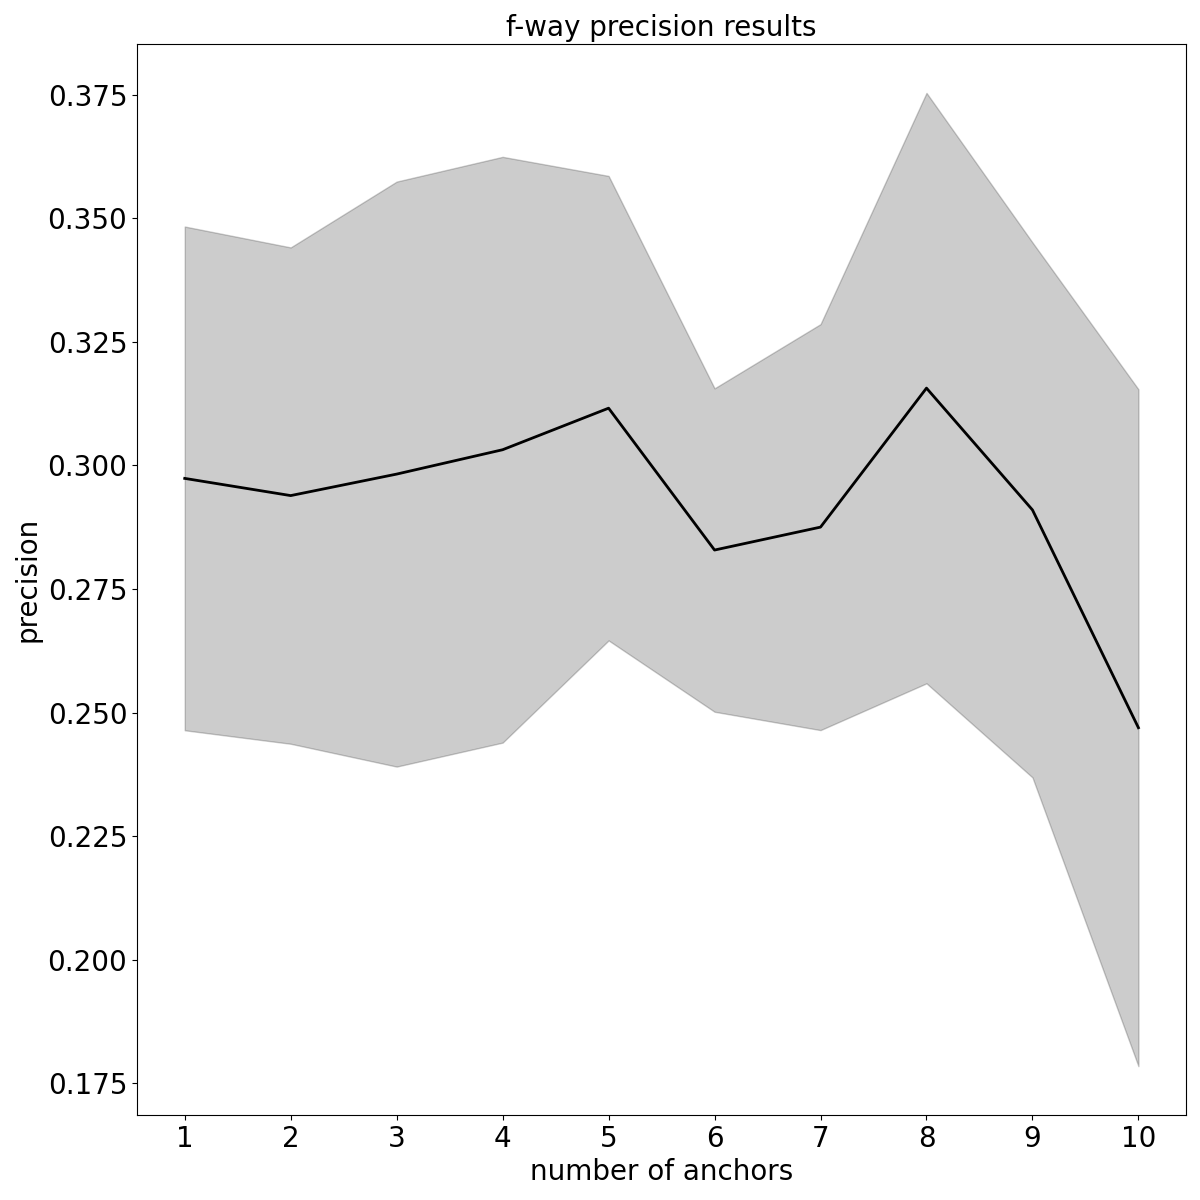
\includegraphics[width=0.65\textwidth]{./results/precision_micro_trend_alohaMB.png}
        \vspace*{-0.2cm}
        \caption[ALOHA (M/B only) Family Prediction Precision Micro Trend]{\textBF{Precision Micro Trend} (varying the number of anchor samples used) resulting from the evaluation of the \textBF{ALOHA (M/B only)} implementation on the Malware Family Prediction task. The line represents the \textit{mean} Micro Precision, while the shaded region represents the \textit{standard deviation}. Statistics were computed over 15 evaluation of the same model with different query and anchor samples.}
        \label{fig:alohaMBPrecisionMicroTrend}
    \end{figure}
}

\newcommand{\jointEmbeddingPrecisionMicroTrend}{
    \begin{figure}[H]
        \vspace*{-0.5cm}
        \centering
        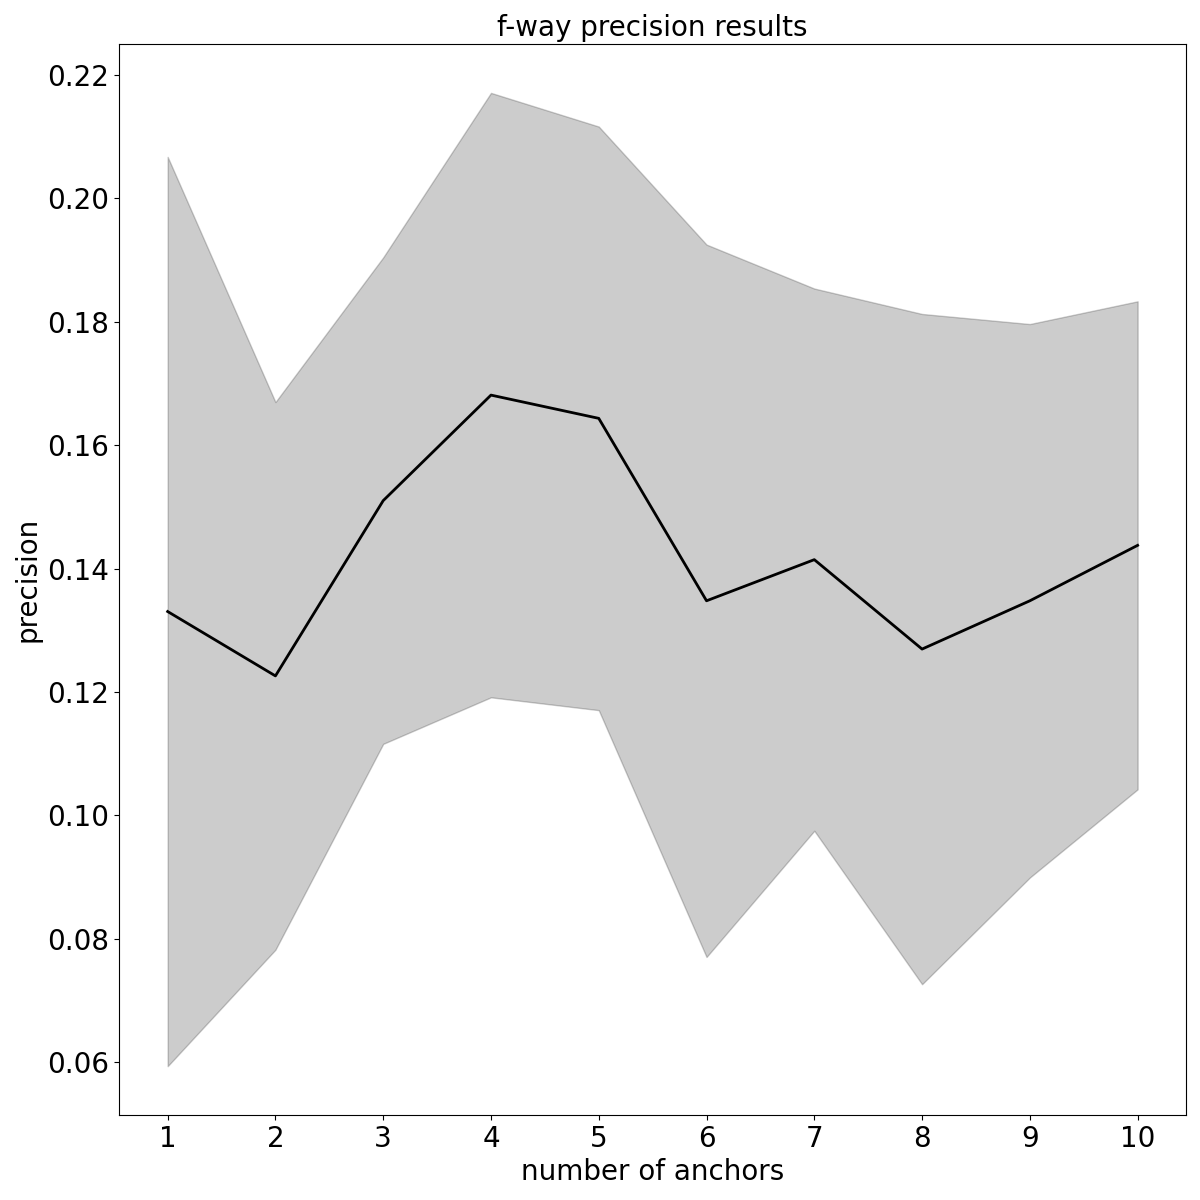
\includegraphics[width=0.65\textwidth]{./results/precision_micro_trend_jointEmbedding.png}
        \vspace*{-0.2cm}
        \caption[Joint Embedding Family Prediction Precision Micro Trend]{\textBF{Precision Micro Trend} (varying the number of anchor samples used) resulting from the evaluation of the \textBF{Joint Embedding} implementation on the Malware Family Prediction task. The line represents the \textit{mean} Micro Precision, while the shaded region represents the \textit{standard deviation}. Statistics were computed over 15 evaluation of the same model with different query and anchor samples.}
        \label{fig:jointEmbeddingPrecisionMicroTrend}
    \end{figure}
}

\newcommand{\proposedModelPrecisionMicroTrend}{
    \begin{figure}[H]
        \vspace*{-0.5cm}
        \centering
        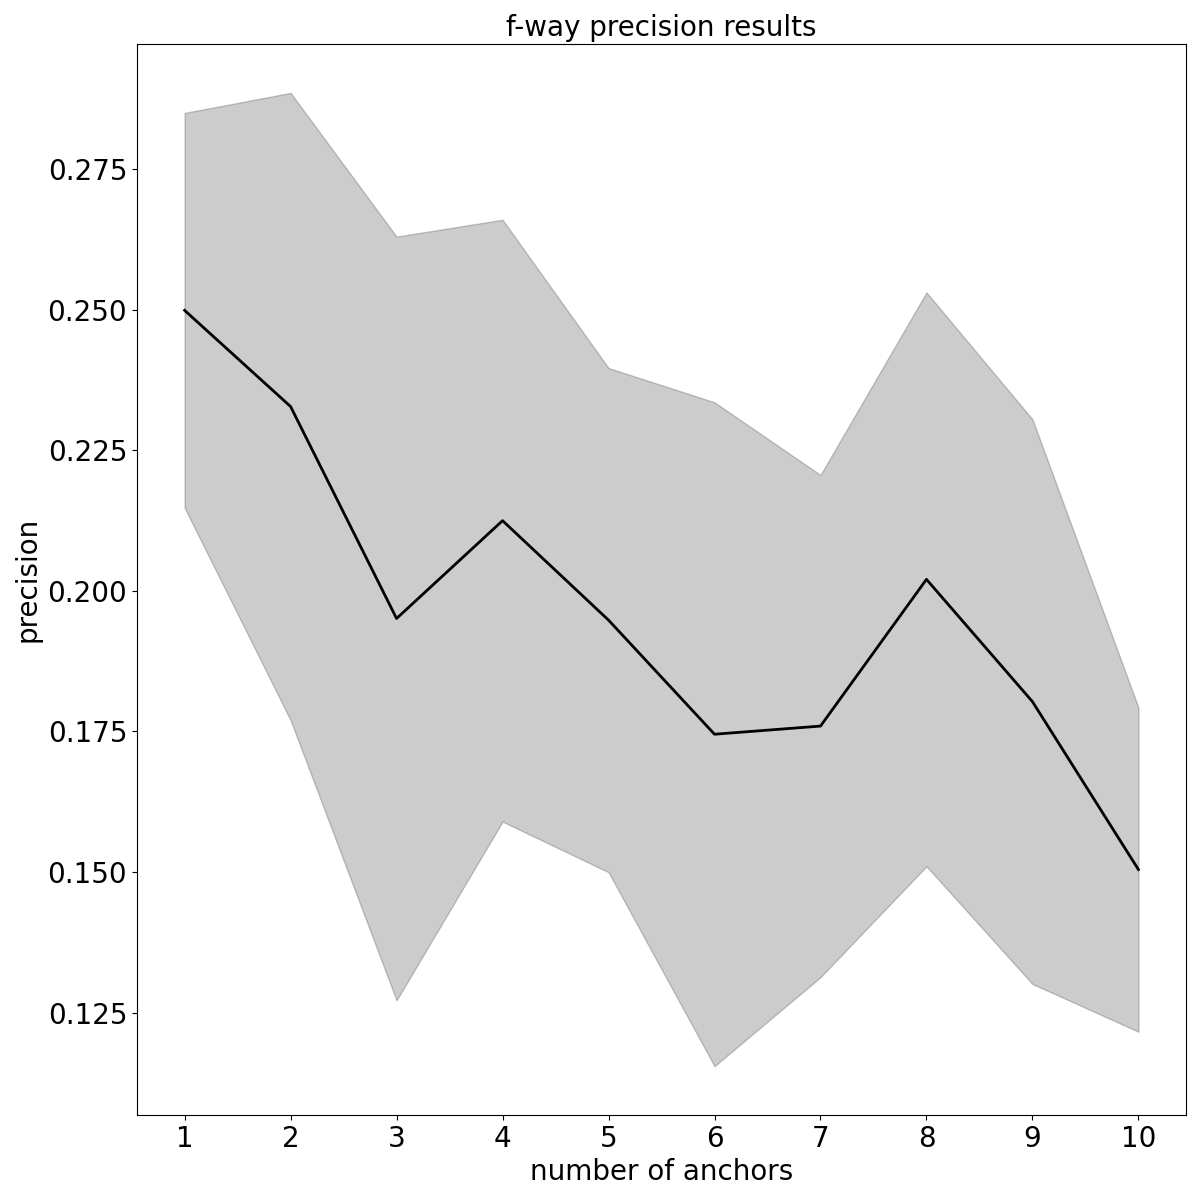
\includegraphics[width=0.65\textwidth]{./results/precision_micro_trend_proposedModel.png}
        \vspace*{-0.2cm}
        \caption[Proposed Model Family Prediction Precision Micro Trend]{\textBF{Precision Micro Trend} (varying the number of anchor samples used) resulting from the evaluation of the \textBF{Proposed Model} implementation on the Malware Family Prediction task. The line represents the \textit{mean} Micro Precision, while the shaded region represents the \textit{standard deviation}. Statistics were computed over 15 evaluation of the same model with different query and anchor samples.}
        \label{fig:proposedModelPrecisionMicroTrend}
    \end{figure}
}

\newcommand{\alohaRecallScoreMacroTrend}{
    \begin{figure}[H]
        \vspace*{-0.5cm}
        \centering
        \includegraphics[width=0.65\textwidth]{./results/recall_score_macro_trend_aloha.png}
        \vspace*{-0.2cm}
        \caption[ALOHA Family Prediction Recall Macro Trend]{\textBF{Recall Macro Trend} (varying the number of anchor samples used) resulting from the evaluation of the \textBF{ALOHA} implementation on the Malware Family Prediction task. The line represents the \textit{mean} Macro Recall, while the shaded region represents the \textit{standard deviation}. Statistics were computed over 15 evaluation of the same model with different query and anchor samples.}
        \label{fig:alohaRecallScoreMacroTrend}
    \end{figure}
}

\newcommand{\alohaMBRecallScoreMacroTrend}{
    \begin{figure}[H]
        \vspace*{-0.5cm}
        \centering
        \includegraphics[width=0.65\textwidth]{./results/recall_score_macro_trend_alohaMB.png}
        \vspace*{-0.2cm}
        \caption[ALOHA (M/B only) Family Prediction Recall Macro Trend]{\textBF{Recall Macro Trend} (varying the number of anchor samples used) resulting from the evaluation of the \textBF{ALOHA (M/B only)} implementation on the Malware Family Prediction task. The line represents the \textit{mean} Macro Recall, while the shaded region represents the \textit{standard deviation}. Statistics were computed over 15 evaluation of the same model with different query and anchor samples.}
        \label{fig:alohaMBRecallScoreMacroTrend}
    \end{figure}
}

\newcommand{\jointEmbeddingRecallScoreMacroTrend}{
    \begin{figure}[H]
        \vspace*{-0.5cm}
        \centering
        \includegraphics[width=0.65\textwidth]{./results/recall_score_macro_trend_jointEmbedding.png}
        \vspace*{-0.2cm}
        \caption[Joint Embedding Family Prediction Recall Macro Trend]{\textBF{Recall Macro Trend} (varying the number of anchor samples used) resulting from the evaluation of the \textBF{Joint Embedding} implementation on the Malware Family Prediction task. The line represents the \textit{mean} Macro Recall, while the shaded region represents the \textit{standard deviation}. Statistics were computed over 15 evaluation of the same model with different query and anchor samples.}
        \label{fig:jointEmbeddingRecallScoreMacroTrend}
    \end{figure}
}

\newcommand{\proposedModelRecallScoreMacroTrend}{
    \begin{figure}[H]
        \vspace*{-0.5cm}
        \centering
        \includegraphics[width=0.65\textwidth]{./results/recall_score_macro_trend_proposedModel.png}
        \vspace*{-0.2cm}
        \caption[Proposed Model Family Prediction Recall Macro Trend]{\textBF{Recall Macro Trend} (varying the number of anchor samples used) resulting from the evaluation of the \textBF{Proposed Model} implementation on the Malware Family Prediction task. The line represents the \textit{mean} Macro Recall, while the shaded region represents the \textit{standard deviation}. Statistics were computed over 15 evaluation of the same model with different query and anchor samples.}
        \label{fig:proposedModelRecallScoreMacroTrend}
    \end{figure}
}

\newcommand{\alohaRecallScoreMicroTrend}{
    \begin{figure}[H]
        \vspace*{-0.5cm}
        \centering
        \includegraphics[width=0.65\textwidth]{./results/recall_score_micro_trend_aloha.png}
        \vspace*{-0.2cm}
        \caption[ALOHA Family Prediction Recall Micro Trend]{\textBF{Recall Micro Trend} (varying the number of anchor samples used) resulting from the evaluation of the \textBF{ALOHA} implementation on the Malware Family Prediction task. The line represents the \textit{mean} Micro Recall, while the shaded region represents the \textit{standard deviation}. Statistics were computed over 15 evaluation of the same model with different query and anchor samples.}
        \label{fig:alohaRecallScoreMicroTrend}
    \end{figure}
}

\newcommand{\alohaMBRecallScoreMicroTrend}{
    \begin{figure}[H]
        \vspace*{-0.5cm}
        \centering
        \includegraphics[width=0.65\textwidth]{./results/recall_score_micro_trend_alohaMB.png}
        \vspace*{-0.2cm}
        \caption[ALOHA (M/B only) Family Prediction Recall Micro Trend]{\textBF{Recall Micro Trend} (varying the number of anchor samples used) resulting from the evaluation of the \textBF{ALOHA (M/B only)} implementation on the Malware Family Prediction task. The line represents the \textit{mean} Micro Recall, while the shaded region represents the \textit{standard deviation}. Statistics were computed over 15 evaluation of the same model with different query and anchor samples.}
        \label{fig:alohaMBRecallScoreMicroTrend}
    \end{figure}
}

\newcommand{\jointEmbeddingRecallScoreMicroTrend}{
    \begin{figure}[H]
        \vspace*{-0.5cm}
        \centering
        \includegraphics[width=0.65\textwidth]{./results/recall_score_micro_trend_jointEmbedding.png}
        \vspace*{-0.2cm}
        \caption[Joint Embedding Family Prediction Recall Micro Trend]{\textBF{Recall Micro Trend} (varying the number of anchor samples used) resulting from the evaluation of the \textBF{Joint Embedding} implementation on the Malware Family Prediction task. The line represents the \textit{mean} Micro Recall, while the shaded region represents the \textit{standard deviation}. Statistics were computed over 15 evaluation of the same model with different query and anchor samples.}
        \label{fig:jointEmbeddingRecallScoreMicroTrend}
    \end{figure}
}

\newcommand{\proposedModelRecallScoreMicroTrend}{
    \begin{figure}[H]
        \vspace*{-0.5cm}
        \centering
        \includegraphics[width=0.65\textwidth]{./results/recall_score_micro_trend_proposedModel.png}
        \vspace*{-0.2cm}
        \caption[Proposed Model Family Prediction Recall Micro Trend]{\textBF{Recall Micro Trend} (varying the number of anchor samples used) resulting from the evaluation of the \textBF{Proposed Model} implementation on the Malware Family Prediction task. The line represents the \textit{mean} Micro Recall, while the shaded region represents the \textit{standard deviation}. Statistics were computed over 15 evaluation of the same model with different query and anchor samples.}
        \label{fig:proposedModelRecallScoreMicroTrend}
    \end{figure}
}

\newcommand{\alohaConfMatrixMaxAcc}{
    \begin{figure}[H]
        \vspace*{-0.5cm}
        \centering
        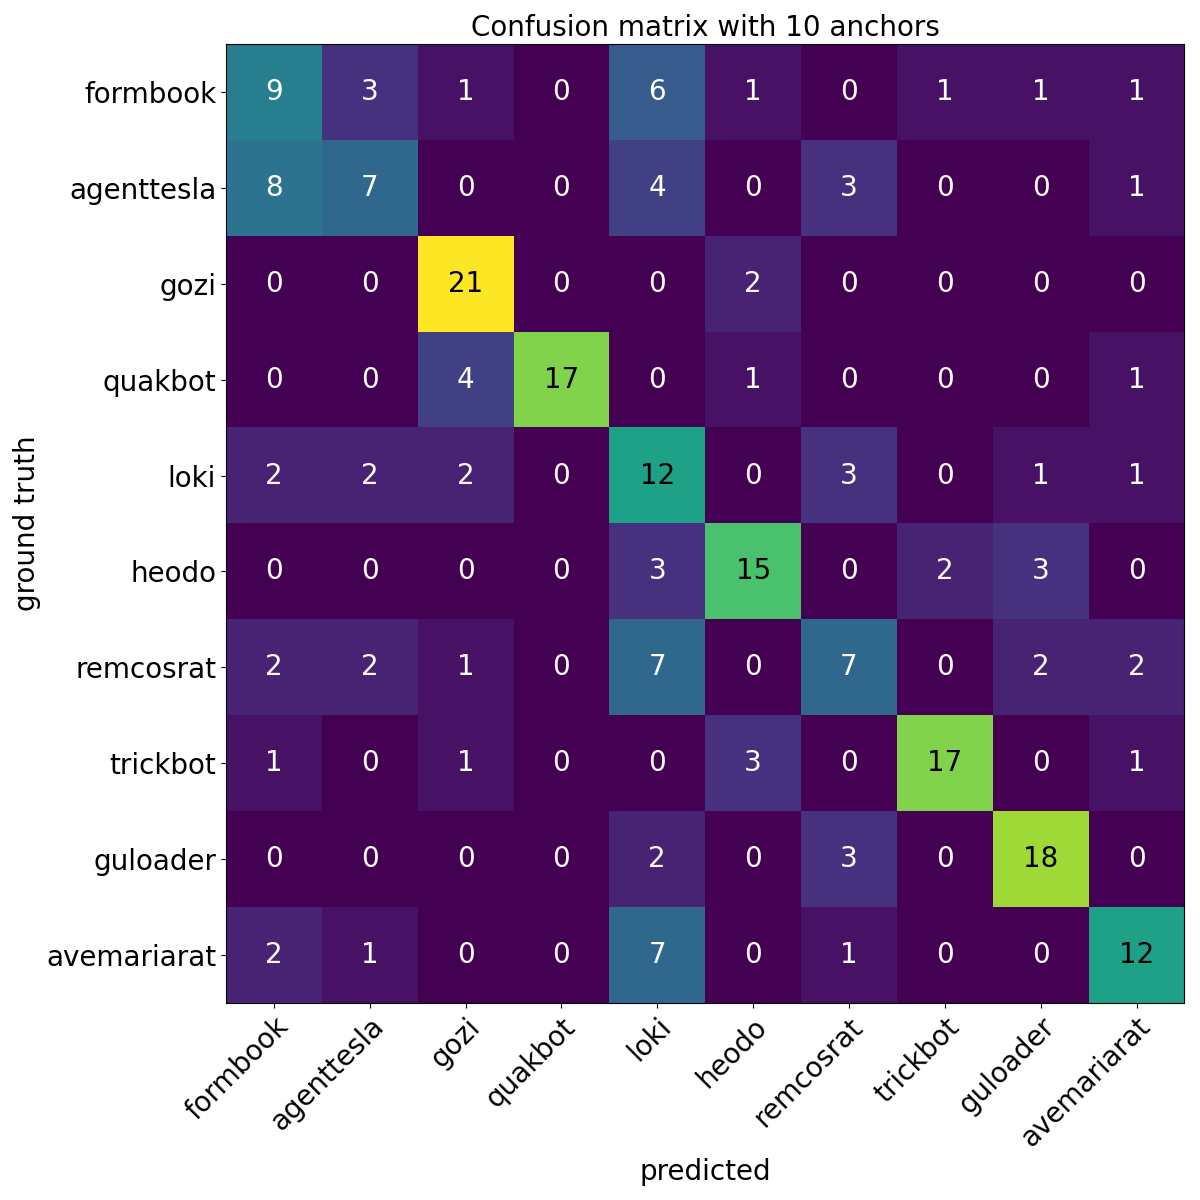
\includegraphics[width=0.65\textwidth]{./results/conf_matrix_max_acc_aloha.png}
        \vspace*{-0.2cm}
        \caption[ALOHA Family Prediction Max Accuracy Confusion Matrix]{\textBF{Confusion Matrix} corresponding to the best prediction when using the number $k$ of anchors which produced the overall best accuracy, resulting from the evaluation of the \textBF{ALOHA} implementation on the Malware Family Prediction task.}
        \label{fig:alohaConfMatrixMaxAcc}
    \end{figure}
}

\newcommand{\alohaMBConfMatrixMaxAcc}{
    \begin{figure}[H]
        \vspace*{-0.5cm}
        \centering
        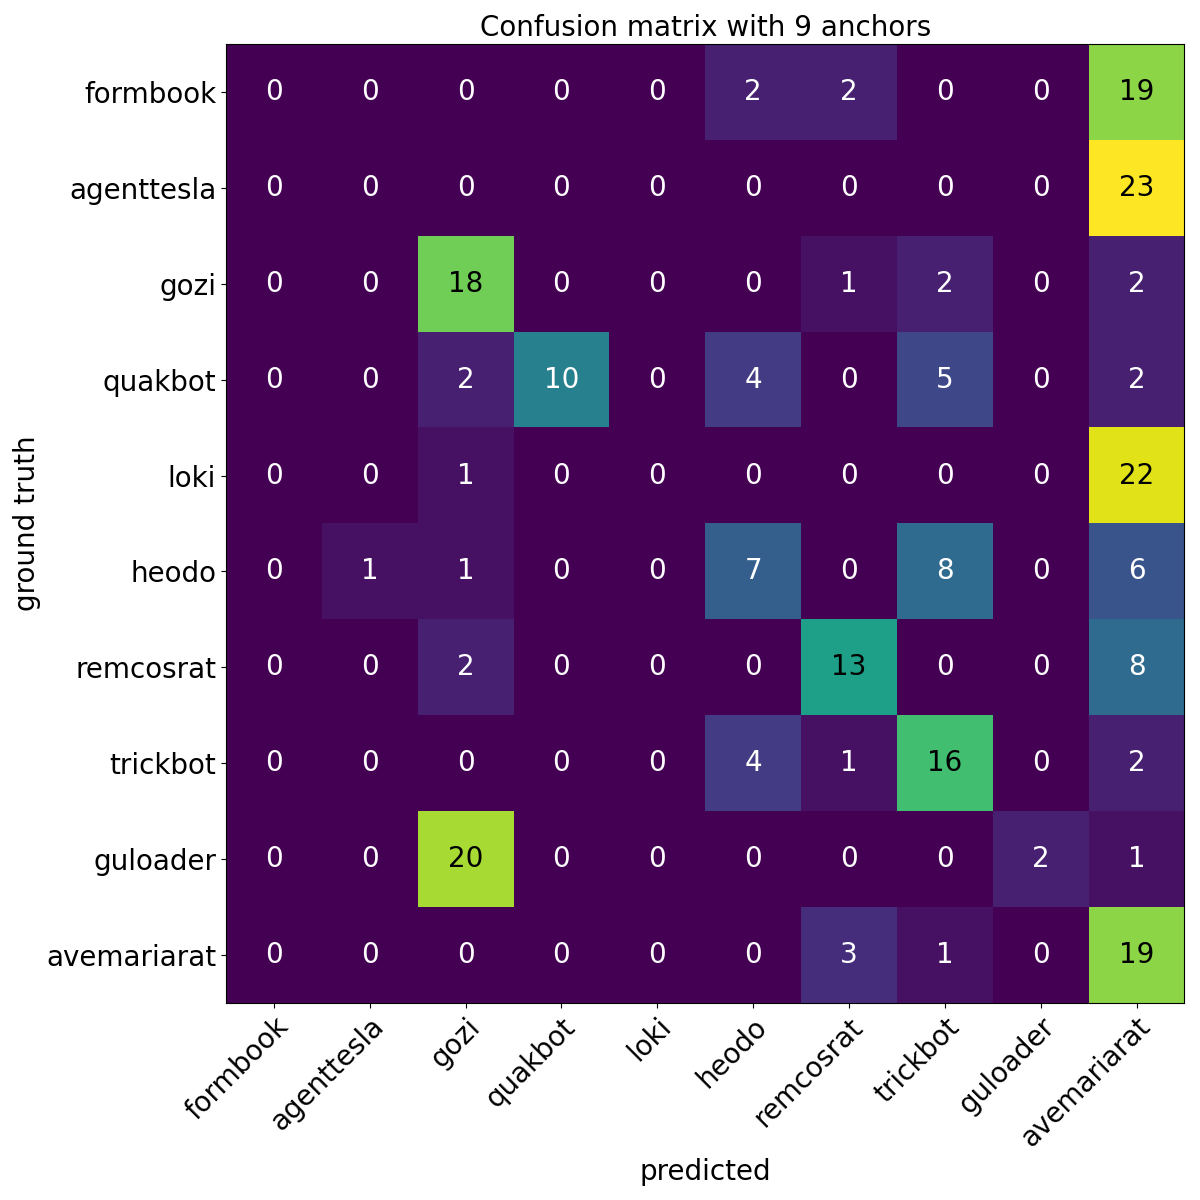
\includegraphics[width=0.65\textwidth]{./results/conf_matrix_max_acc_alohaMB.png}
        \vspace*{-0.2cm}
        \caption[ALOHA (M/B only) Family Prediction Max Accuracy Confusion Matrix]{\textBF{Confusion Matrix} corresponding to the best prediction when using the number $k$ of anchors which produced the overall best accuracy, resulting from the evaluation of the \textBF{ALOHA (M/B only)} implementation on the Malware Family Prediction task.}
        \label{fig:alohaMBConfMatrixMaxAcc}
    \end{figure}
}

\newcommand{\jointEmbeddingConfMatrixMaxAcc}{
    \begin{figure}[H]
        \vspace*{-0.5cm}
        \centering
        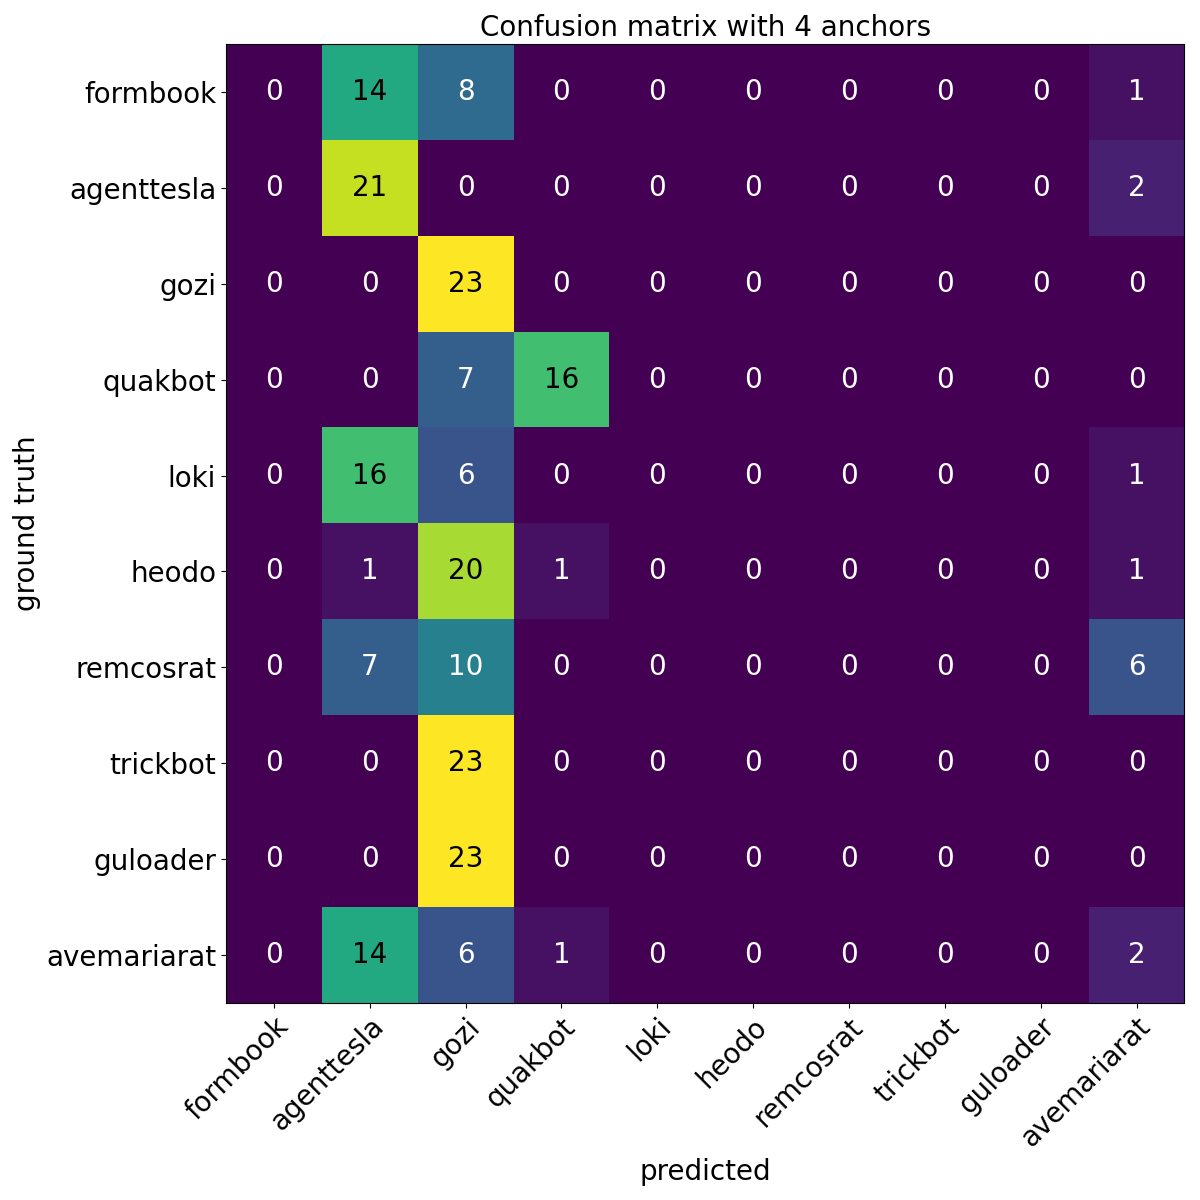
\includegraphics[width=0.65\textwidth]{./results/conf_matrix_max_acc_jointEmbedding.png}
        \vspace*{-0.2cm}
        \caption[Joint Embedding Family Prediction Max Accuracy Confusion Matrix]{\textBF{Confusion Matrix} corresponding to the best prediction when using the number $k$ of anchors which produced the overall best accuracy, resulting from the evaluation of the \textBF{Joint Embedding} implementation on the Malware Family Prediction task.}
        \label{fig:jointEmbeddingConfMatrixMaxAcc}
    \end{figure}
}

\newcommand{\proposedModelConfMatrixMaxAcc}{
    \begin{figure}[H]
        \vspace*{-0.5cm}
        \centering
        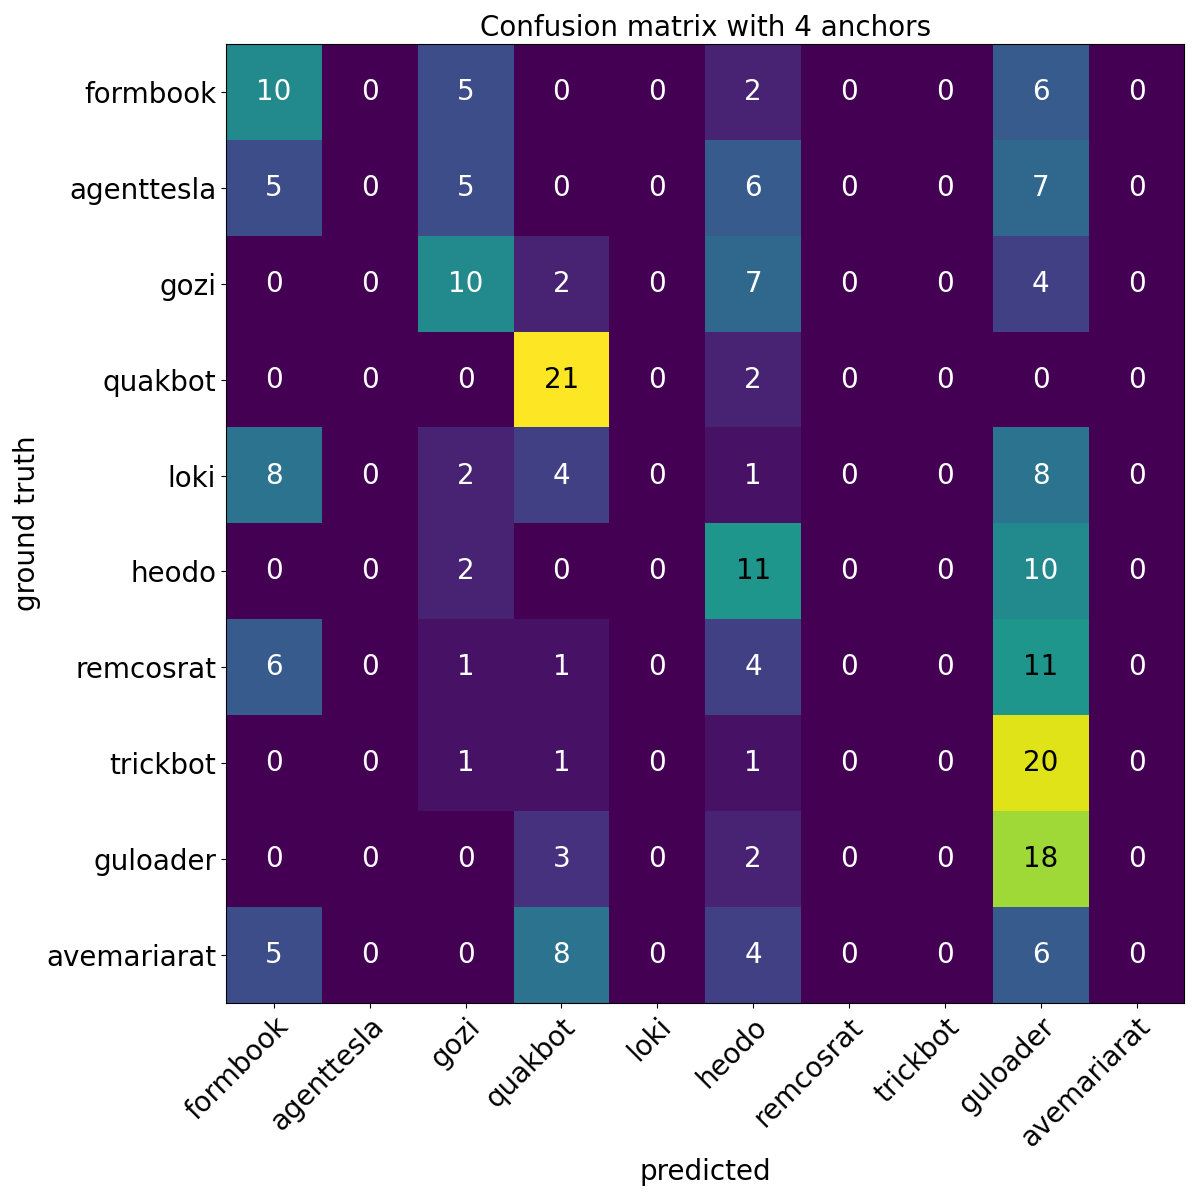
\includegraphics[width=0.65\textwidth]{./results/conf_matrix_max_acc_proposedModel.png}
        \vspace*{-0.2cm}
        \caption[Proposed Model Family Prediction Max Accuracy Confusion Matrix]{\textBF{Confusion Matrix} corresponding to the best prediction when using the number $k$ of anchors which produced the overall best accuracy, resulting from the evaluation of the \textBF{Proposed Model} implementation on the Malware Family Prediction task.}
        \label{fig:proposedModelConfMatrixMaxAcc}
    \end{figure}
}

\newcommand{\alohaConfMatrixMinAcc}{
    \begin{figure}[H]
        \vspace*{-0.5cm}
        \centering
        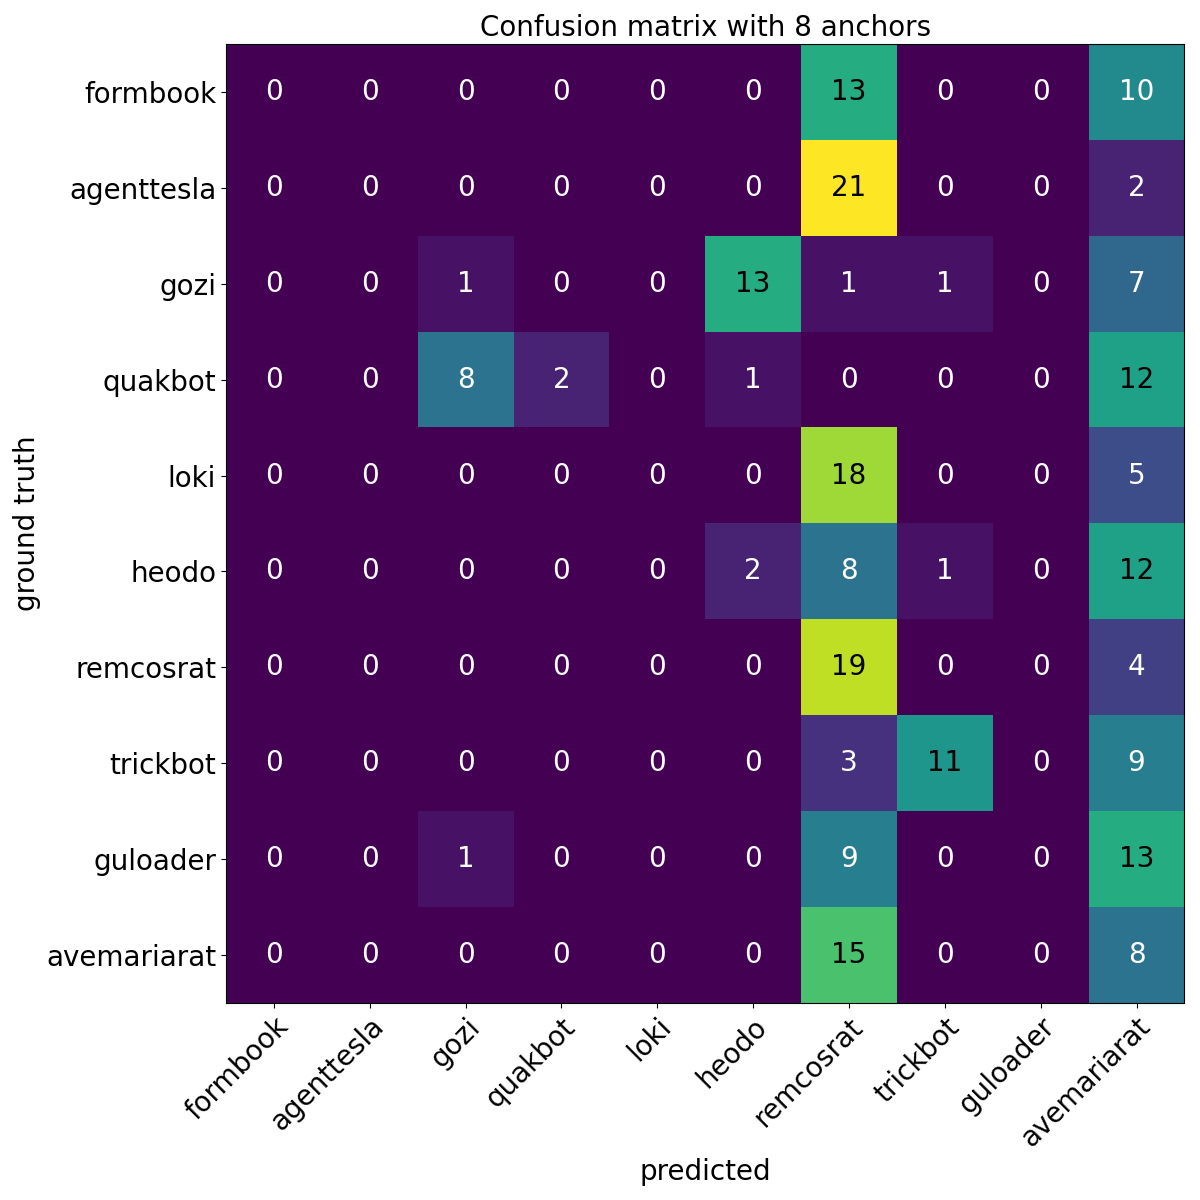
\includegraphics[width=0.65\textwidth]{./results/conf_matrix_min_acc_aloha.png}
        \vspace*{-0.2cm}
        \caption[ALOHA Family Prediction Min Accuracy Confusion Matrix]{\textBF{Confusion Matrix} corresponding to the worst prediction when using the number $k$ of anchors which produced the overall best accuracy, resulting from the evaluation of the \textBF{ALOHA} implementation on the Malware Family Prediction task.}
        \label{fig:alohaConfMatrixMinAcc}
    \end{figure}
}

\newcommand{\alohaMBConfMatrixMinAcc}{
    \begin{figure}[H]
        \vspace*{-0.5cm}
        \centering
        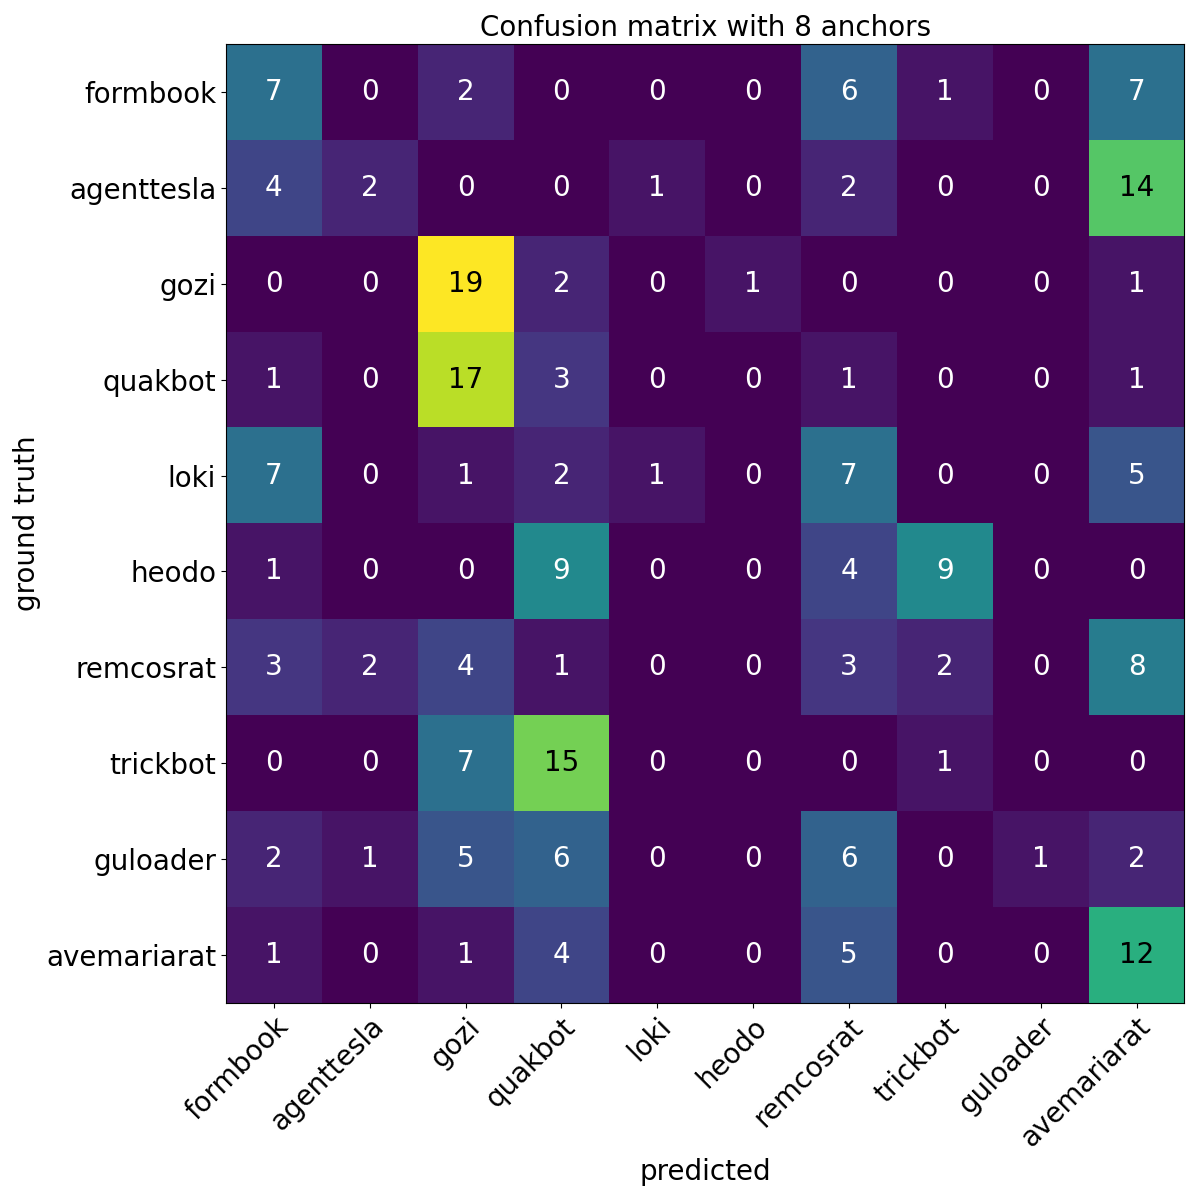
\includegraphics[width=0.65\textwidth]{./results/conf_matrix_min_acc_alohaMB.png}
        \vspace*{-0.2cm}
        \caption[ALOHA (M/B only) Family Prediction Min Accuracy Confusion Matrix]{\textBF{Confusion Matrix} corresponding to the worst prediction when using the number $k$ of anchors which produced the overall best accuracy, resulting from the evaluation of the \textBF{ALOHA (M/B only)} implementation on the Malware Family Prediction task.}
        \label{fig:alohaMBConfMatrixMinAcc}
    \end{figure}
}

\newcommand{\jointEmbeddingConfMatrixMinAcc}{
    \begin{figure}[H]
        \vspace*{-0.5cm}
        \centering
        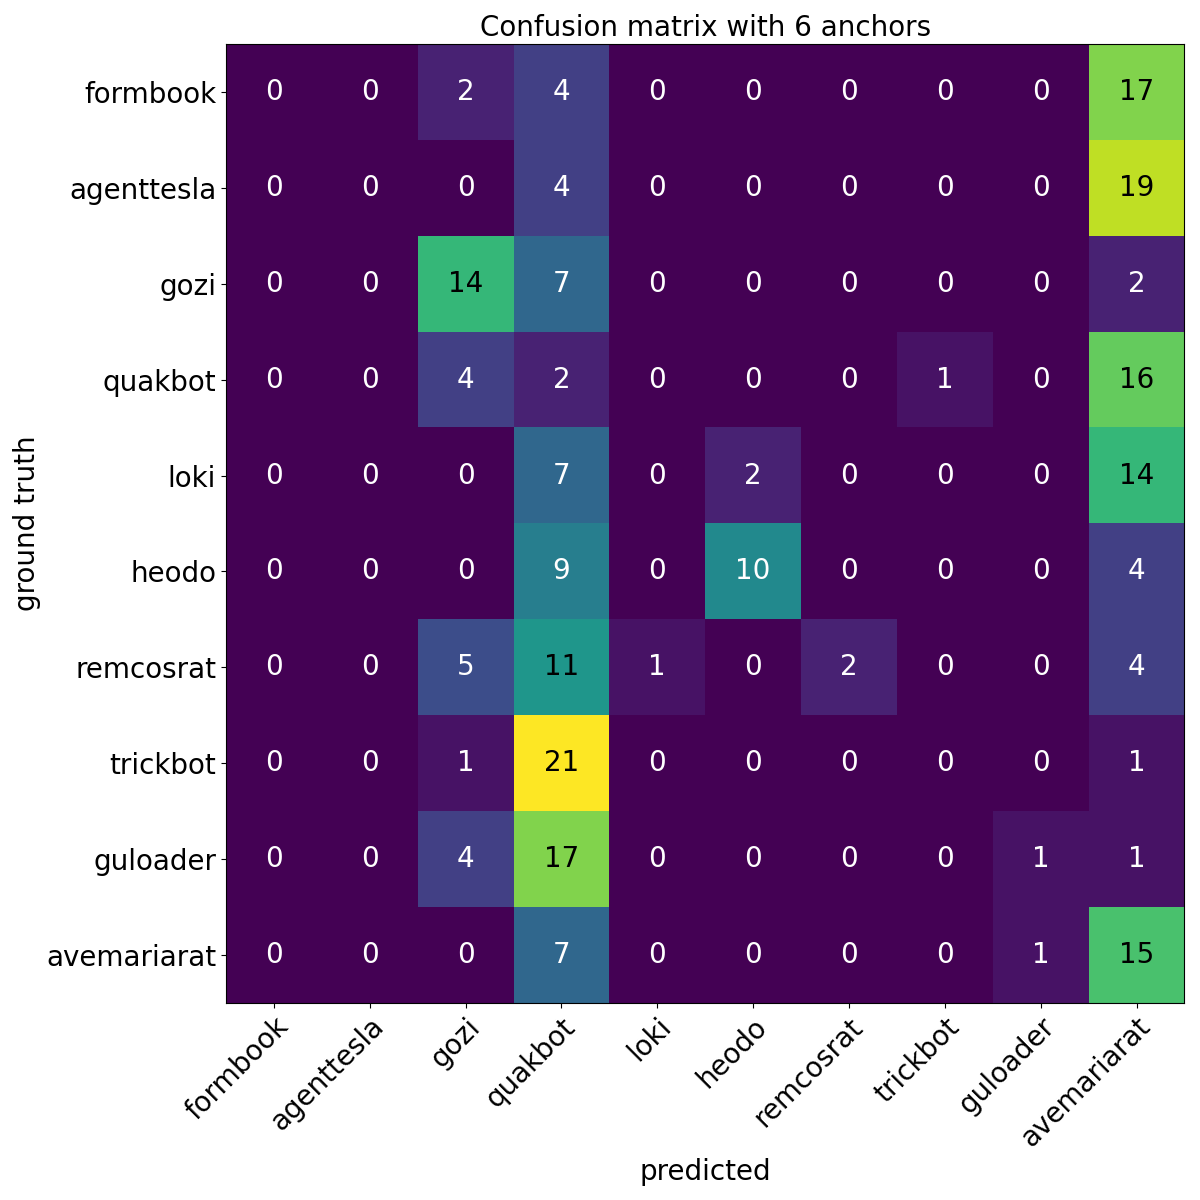
\includegraphics[width=0.65\textwidth]{./results/conf_matrix_min_acc_jointEmbedding.png}
        \vspace*{-0.2cm}
        \caption[Joint Embedding Family Prediction Min Accuracy Confusion Matrix]{\textBF{Confusion Matrix} corresponding to the worst prediction when using the number $k$ of anchors which produced the overall best accuracy, resulting from the evaluation of the \textBF{Joint Embedding} implementation on the Malware Family Prediction task.}
        \label{fig:jointEmbeddingConfMatrixMinAcc}
    \end{figure}
}

\newcommand{\proposedModelConfMatrixMinAcc}{
    \begin{figure}[H]
        \vspace*{-0.5cm}
        \centering
        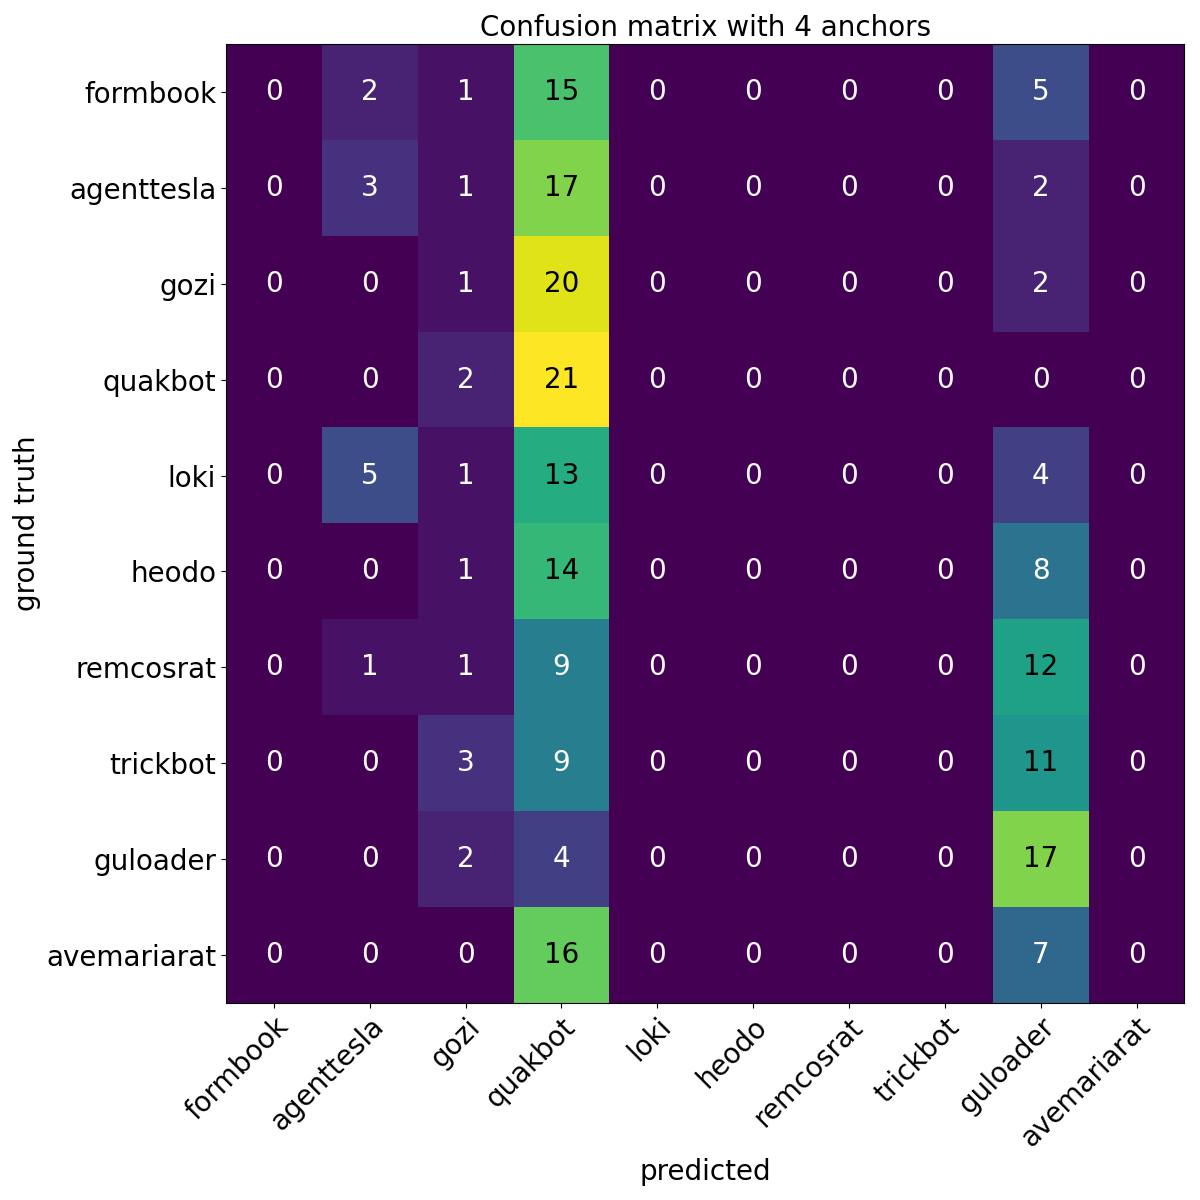
\includegraphics[width=0.65\textwidth]{./results/conf_matrix_min_acc_proposedModel.png}
        \vspace*{-0.2cm}
        \caption[Proposed Model Family Prediction Min Accuracy Confusion Matrix]{\textBF{Confusion Matrix} corresponding to the worst prediction when using the number $k$ of anchors which produced the overall best accuracy, resulting from the evaluation of the \textBF{Proposed Model} implementation on the Malware Family Prediction task.}
        \label{fig:proposedModelConfMatrixMinAcc}
    \end{figure}
}

